%======================================================
\chapter{Numerical Solution Strategy}\label{chap:rt-numerical-strategy}
%======================================================


%---------------------------------------------
\section{Discretization of Frequencies}
%---------------------------------------------


The moments of the equation of radiative transfer, given in
eqns.~\ref{eq:dEdt-freq}~-~\ref{eq:dFdt-freq}, are still frequency specific, and would need to be
solved for each frequency between 0 Hz and infinity individually. This is obviously not a feasible
approach. Instead, these equations need to be discretized in frequency first. I follow the approach
of \cite{ramses-rt13} and for a rough approximation of multi-frequency, a relevant frequency range
is split into a number $M$ of mutually exclusive groups of frequency ranges:

\begin{align}
	& [\nu_{00}, \nu_{01}\ : \ \nu_{10}, \nu_{11}\ : ... \ : \ \nu_{M0}, \nu_{M1}\ ] =
        [\nu_{0}, \infty [
\end{align}

The frequency ranges are chosen to be convenient for us. Specifically, since the interaction cross
sections of ionizing species are zero below the ionizing frequency of their corresponding species,
it makes sense to use the various ionizing frequencies as the boundaries for the frequency groups.
Since the prime interest in the cosmological context is to heat and ionize the gas, it makes little
sense to keep track of photons with frequencies below the smallest ionizing frequency. So in
practice the lower threshold $\nu_0$ is usually the hydrogen ionization frequency given in
eq.~\ref{eq:nuIonHI}. (The interaction cross sections are all zero below that threshold anyway.)
However if effects like radiation pressure are included, then the relevant frequency range is in
the infrared spectrum, and the $\nu_0$ is lower than the hydrogen ionization frequency, which is in
the ultraviolet frequency range. Additionally, frequencies below the lowest interaction threshold
are of interest when Doppler effects due to the relative motion of the gas are accounted for, which
we also neglect for now.

Rather than treating the photon energy densities and fluxes for individual frequencies, we now use
their integrated averages over a frequency group. For any frequency group $i$, we have

\begin{align}
	E_i &=
        \int\limits_{\nu_{i0}}^{\nu_{i1}} E_\nu d\nu \\
	\Fbf_i &=
       \int\limits_{\nu_{i0}}^{\nu_{i1}} \Fbf_\nu d\nu
\end{align}


giving us the following discretized equations to solve:


\begin{align}
	\DELDT{E_i} + \nabla \cdot \Fbf_i &=
		- \sum\limits_{j}^{\absorbers} n_j \sigma_{i j}^N c E_i + \dot{E}_i^* + \dot{E}_i ^{rec}
		\label{eq:dEdt-group} \\
	\DELDT{\Fbf_i} + c^2 \ \nabla \cdot \mathds{P}_i &=
		- \sum\limits_{j}^{\absorbers} n_j \sigma_{i j}^N c \Fbf_i
		\label{eq:dFdt-group}
\end{align}


The expression for the number weighted average cross section $\sigma_{ij}^N$ is given in eq.
\ref{eq:sigma_N}. The radiation pressure tensor is discretized in the same manner:

\begin{align}
	\mathds{P}_i &=
        \mathds{D}_i E_i \label{eq:pressure-tensor-group-start}\\
	\mathds{D}_i &=
        \frac{1- \chi_i}{2} \mathds{I} + \frac{3 \chi_i - 1}{2} \mathbf{n}_i \otimes \mathbf{n}_i
        \label{eq:eddington-group} \\
	\mathbf{n}_i &=
        \frac{\Fbf_i}{|\Fbf_i|} \\
	\chi_i &=
        \frac{3 + 4 f_i ^2}{5 + 2 \sqrt{4 - 3 f_i^2}} \\
	f_i &=
        \frac{|\Fbf_i|}{c E_i} \label{eq:pressure-tensor-group-end}
\end{align}



For the computation of the  photo-heating and photo-ionization rates, we need to introduce the mean
photon energy $\overline{\epsilon}_i$ of the frequency bin $i$. In order to estimate the average
energy over a frequency interval, the distribution of the radiation energy over the frequencies,
i.e. the photon spectrum, needs to be known. Unfortunately, the exact spectrum of the radiation
field can't be known without tracing the frequencies individually, as the initially emitted spectrum
changes over time due to frequency dependent interactions with the gas. In addition, if radiation
sources with different spectra are present, the superposition of the radiation stemming from these
varying sources would change the local spectrum of the radiation as well. So the exact spectrum
needs to be approximated with a guess. \cite{ramses-rt13} recommend taking an average value among
all stellar radiation sources. In this work, I assume a blackbody spectrum, which for a temperature
$T$ is given by:

\begin{align}
    \mathcal{J}_\nu(T) = \frac{2 \nu^2}{c^2} \frac{h \nu}{\exp\left(h\nu/k_B T\right) - 1} \ .
    \label{eq:blackbody}
\end{align}

The temperature $T$ in this case would be some effective temperature for stellar sources, not the
local temperature of the gas. With an assumed spectral shape, the mean photon energy
$\overline{\epsilon}_i$ in each frequency group $i$ can be estimated as


\begin{align}
\overline{\epsilon}_i \equiv
    \frac{E_i}{N_i} =
    \frac{
        \int\limits_{\nu_{i0}}^{\nu_{i1}} E_\nu \ d\nu
        }{
        \int\limits_{\nu_{i0}}^{\nu_{i1}} N_\nu \ d\nu
        }
    \approx
    \frac{
        \int\limits_{\nu_{i0}}^{\nu_{i1}} \mathcal{J}_\nu \ d\nu
        }{
        \int\limits_{\nu_{i0}}^{\nu_{i1}} \mathcal{J}_\nu / h\nu \ d\nu
        }
\end{align}

Using the mean photon energy $\overline{\epsilon}_i$, the photo-heating rate $\mathcal{H}_{i,j}$
of the gas for the photon group $i$ and ionizing species $j$ then becomes:

\begin{align}
\mathcal{H}_{i, j} &=
\left[
		\int\limits_{\nu_{i0}}^{\nu_{i1}}\de \nu h \nu N_\nu  \sigma_{j\nu} -
	h \nu_{ion,j}\
		\int\limits_{\nu_{i0}}^{\nu_{i1}}\de \nu N_\nu \sigma_{j\nu} \
\right] \ c \ n_j \\
%
&=
\left[
	\sigma_{ij}^E E_i - h \nu_{ion,j}\ \sigma_{ij}^N N_i
\right]  c \ n_j \\
&=
\left[
	\sigma_{ij}^E \overline{\epsilon}_i - h \nu_{ion,j}\ \sigma_{ij}^N
\right]  N_i\ c \ n_j \\
&=
\left[
	\sigma_{ij}^E  - h \nu_{ion,j}\ \sigma_{ij}^N /\ \overline{\epsilon}_i
\right]  E_i\ c \ n_j
\label{eq:photoheating-group}
\end{align}




And the photo-ionization rate can be written as

\begin{align}
\Gamma_{i, j}
	&=
		c \ \int\limits_{\nu_{i0}}^{\nu_{i1}}\de \nu \ \sigma_{\nu j} N_\nu \\
	&= c \ \sigma_{ij}^N N_i
	= c \ \sigma_{ij}^N E_i / \overline{\epsilon}_i \label{eq:photoionization-group}
\end{align}


Finally, the photon absorption (destruction) rates for a frequency bin $i$ and ionizing species $j$
are given by

\begin{align}
\DELDT{E_i} &=
    \deldt{(N_i \ \overline{\epsilon}_i)} =
    \overline{\epsilon}_i \DELDT{N_i} =
    -\overline{\epsilon}_i c \ \sigma_{i j} ^ N n_j
\end{align}


Here we have introduced the number- and energy-weighted average cross sections:
\begin{align}
\sigma_{ij}^N &=
		\frac{
			\int\limits_{\nu_{i0}}^{\nu_{i1}}\de \nu \ N_\nu \ \sigma_{j\nu}
		} {
		  \int\limits_{\nu_{i0}}^{\nu_{i1}}\de \nu \ N_\nu
		}
		\approx
		\frac{
			\int\limits_{\nu_{i0}}^{\nu_{i1}}\de \nu \ \mathcal{J}(\nu) / (h \ \nu) \sigma_{j\nu}
		} {
  		\int\limits_{\nu_{i0}}^{\nu_{i1}}\de \nu \ \mathcal{J}(\nu) / (h \ \nu)
		} \label{eq:sigma_N}\\
\sigma_{ij}^E &=
		\frac{
			\int\limits_{\nu_{i0}}^{\nu_{i1}}\de \nu \ h \nu N_\nu \ \sigma_{j\nu}
		}	{
			\int\limits_{\nu_{i0}}^{\nu_{i1}}\de \nu \ h \nu N_\nu
		}
		\approx
		\frac{
			\int\limits_{\nu_{i0}}^{\nu_{i1}}\de \nu \ \mathcal{J}(\nu) \  \sigma_{j\nu}
		}	{
			\int\limits_{\nu_{i0}}^{\nu_{i1}}\de \nu \ \mathcal{J}(\nu)
		} \label{eq:sigma_E}
\end{align}








%---------------------------------------------
\section{One RT Time Step}
%---------------------------------------------



%---------------------------------------------
\subsection{Outline}\label{chap:rt-numerics-outline}
%---------------------------------------------


For each photon frequency group, the equations \ref{eq:dEdt-group} and \ref{eq:dFdt-group} are
solved with an operator-splitting strategy. Following the approach of \cite{ramses-rt13}, the
equations are decomposed into three steps that are executed in sequence over the same time step
$\Delta t$:

\begin{enumerate}

\item \textbf{Photon injection step}: the radiation from radiative sources is injected into the
grid.

\item \textbf{Photon transport step}: Photons are transported in space by solving the homogenized
equations \ref{eq:dEdt-group} and \ref{eq:dFdt-group}, i.e. the right hand side of these equations
is set to zero.

\item \textbf{Thermochemistry step}: The rest of the source terms (the right hand side) of the
equations \ref{eq:dEdt-group} and \ref{eq:dFdt-group} is solved.
\end{enumerate}

In what follows, the numerical and algorithmic aspects of these three steps are discussed
individually. But first, we should look at the broader picture and discuss some fundamentals upon
which the RT scheme will be built.









%-------------------------------------------------------
\subsubsection{Coupling to Hydrodynamics}
%-------------------------------------------------------

As mentioned before, the effects of radiation on the gas act as source terms for the Euler equations
(eq.~\ref{eq:euler-equations}). Let $\mathcal{S}_{RT}$ denote the source term stemming from the
radiation. Then, neglecting all other source terms, the Euler equations can be written as

\begin{align}
    \DELDT{\U} + \nabla \cdot \F = \mathcal{S}_{RT}
\end{align}

Let $H(\Delta t)$ denote the operator that solves the homogenized (i.e. source-free) part of the
equation over some time step $\Delta t$,

\begin{align}
  H(\Delta t) [\U]: \quad \text{Get }\U(t+\Delta t) \text{ according to } \DELDT{\U} + \nabla \cdot
\F = 0
\end{align}

Similarly, let $S(\Delta t)$ denote the operator that solves only the source part of the equation
over some time step $\Delta t$:

\begin{align}
  S(\Delta t) [\U]: \quad \text{Get }\U(t+\Delta t) \text{ according to } \DELDT{\U} =
\mathcal{S}_{RT}
\end{align}

The operator splitting approach consists of solving the homogenized and the source part of the
equation in sequence rather than concurrently, and the full solution of the system at time $t +
\Delta t$ is given by

\begin{align}
    \U(t+\Delta t) = S(\Delta t)\left[ H(\Delta t) \left[ \U(t) \right] \right] = S(\Delta t) \circ
H(\Delta t) [\U(t)] \label{eq:operator-splitting-hydro-rt}
\end{align}

The solution is first order accurate in time as long as both $H$ and $S$ are also at least first
order accurate operators. In terms of accuracy, the order in which the operators are applied is
inconsequential\footnote{
The analysis of the order of accuracy and interchangeability of operators in operator splitting
techniques, also known as ``fractional-step methods'', relies on the analysis of how the truncation
errors of the used methods behave when the operators are applied in sequence instead of
simultaneously, and what the \emph{numerical} result would look like when using split operators. The
application of a discrete approximate numerical method inevitably leads to error terms being
introduced anyway (see Section~\ref{chap:numerical_diffusion}). The important point is to take into
account whether, and if it does: how the leading order of error terms change when the operators are
split and solved in succession. See \citet{levequeFiniteVolumeMethods2002} for more details.
}, so we can set the order according to our convenience.









%-----------------------------------------------------------------------------
\subsubsection{Using a Particle Based Method: Selecting Reference Frames}
%-----------------------------------------------------------------------------


In contrast to \cite{ramses-rt13}, who use a finite volume method and adaptive mesh refinement to
solve the moments of the equation of radiative transfer, \GEARRT uses a finite volume particle
method, whose derivation and application to the Euler equations was previously discussed in
Part~\ref{part:meshless}. Rather than cells, which are traditionally employed in finite volume
methods, \GEARRT uses particles as discretization elements. The particles, which represent the gas,
are Lagrangian, i.e. are being moved along with the fluid, and have individual time step sizes (see
Section~\ref{chap:individual-timesteps}).
This approach is maintained with \GEARRT: the motion (drifts) of particles is exclusively determined
by the hydrodynamics. The radiative transfer is solved using a different approach by exploiting the
fact that finite volume particle methods are arbitrary Lagrangian-Eulerian, i.e. are valid in both
co-moving and static frames of reference. In the context of RT, the particles are treated as static
interpolation points with respect to the simulated volume, rather than elements co-moving with the
radiation. As such, the particles carry the fluid quantities stored as a co-moving quantity, while
the radiation fields are taken to be in a static frame of reference. This means however that when
particles are drifted, the radiation fields they carry are drifted along as well, which is wrong.
Hence corrections in the radiation fields are necessary when particles are drifted. The exact form
of these corrections will be discussed in Section~\ref{chap:rt-drift}.










%----------------------------------------------------------------------------------
\subsubsection{Setting the Order of Operators to Re-Use Neighbors of Hydrodynamics}
%----------------------------------------------------------------------------------

An essential part of finite volume particle methods is the (repeated) interaction of every particle
with its neighboring particles. To facilitate these interactions, first a neighbor search must be
conducted to determine which particles are ``neighbors'' of each other (see
Section~\ref{chap:meshless-full} for details). This needs to be done each time particle positions
change, i.e. each time particles are drifted. Both the hydrodynamics and the radiative transfer
require the neighbor search to be completed before the actual interactions between particles can
take place. Since the neighbor search is already implemented for the hydrodynamics, and the
particles aren't being drifted in the middle of a simulation step, it is practically convenient to
solve the radiative transfer \emph{after} the hydrodynamics and re-use the existing known neighbors.
Using the operators $S$ and $H$, this means that the solution strategy can be written as:

\begin{align}
    \U(t + \Delta t) = S(\Delta t) \circ H(\Delta t) [ \U (t)] \ .
\end{align}

This equation is the same as eq.~\ref{eq:operator-splitting-hydro-rt}, but here it's intended to
\emph{define} the exact order in which the operators will be solved in \GEARRT.








%-----------------------------------------------------------------------------------
\subsubsection{On the Choice to Treat Radiation in a Static Reference Frame}
%-----------------------------------------------------------------------------------


The approach to treat the radiation in a static frame of reference with respect to the simulated
volume and the hydrodynamics in a Lagrangian one has caveats. For example, sharp discontinuities in
radiation energy densities and photon fluxes will be more diffusive then they could be, as the
particle positions aren't compressed along the front of the discontinuity. A second caveat is that
corrections to the radiation fields are necessary when particles are drifted, as outlined above and
discussed in Section~\ref{chap:rt-drift}. These corrections may in general not be strictly
conservative, as will be shown in Section~\ref{chap:validation-drift-corrections}.

However, the caveats of the approach to treat the radiation in an Eulerian frame of reference and
the hydrodynamics in a Lagrangian one are outweighed by the many advantages it offers. Firstly, the
hydrodynamics remain self-consistent, as the approach can be basically formulated as ``let the
hydrodynamics determine how the hydrodynamics is solved''. The particle positions will trace the
fluid rather than the radiation fields. Secondly, as discussed in the previous section, the
radiation fields are separated into several photon frequency groups. Suppose we decided to make the
particles co-moving with the radiation instead of with the gas. Then the first question would be:
Which frequency group should we choose to determine the particle motion? By treating the particles
as static interpolation points in the context of RT, all frequency groups are treated equally.
Thirdly, it allows us to save a tremendous workload when a sub-cycling approach is applied. The main
idea behind sub-cycling is to somewhat decouple the time integration of the hydrodynamics and the
radiative transfer from each other. In general, radiation, whose signal velocity is always the speed
of light, will require much shorter time step sizes compared to the fluid, with a difference of
several orders of magnitude. The idea is to allow the RT to progress over several (hundreds) of time
steps for each particle individually using its own radiation time step size, while the hydrodynamics
is updated according to its own hydrodynamics time step size. In terms of operators $S$ and $H$, the
sub-cycling can be written as:

\begin{align}
    \U(t + \Delta t) =
        S(\Delta t/n) \circ S(\Delta t/n) \circ ... \circ S(\Delta t/n) \circ H(\Delta t)[\U(t)]
\end{align}

where $n$ sub-cycles with time steps $\Delta t/n$ have been computed for a single homogenized
hydrodynamics operator $H$. Furthermore, just as is the case for hydrodynamics, particles are also
given individual radiation time step sizes (see Section~\ref{chap:individual-timesteps}),
independently of the particles' hydrodynamics time step sizes.

The alternative would be needing to restrict the hydrodynamics time step size to the radiation time
step size, and hence having to perform many hydrodynamics time steps which are in principle not
strictly necessary. Additionally, if particle drifts are performed only according to what the
hydrodynamics prescribe, it means that each RT sub-cycle can proceed without drifting particles, and
hence there is no need for neighbor search interaction loops during RT sub-cycles as well. This
saves a tremendous amount of work, as will be demonstrated in Section~\ref{chap:subcycling-results}. The
sub-cycling approach is discussed in more details in Sections~\ref{chap:dynamic-sybcycling} and \ref{chap:subcycling}.







%----------------------------------------------------------------------
\subsubsection{Summary}
%----------------------------------------------------------------------

Before we continue with the description of each of the operator splitting steps required
for the solution of the radiative transfer described at the beginning of this section, let's
summarize the fundamental approach upon which \GEARRT is built:

\begin{itemize}
\item The basic discretization elements are particles.
\item The underlying method to solve the hyperbolic conservation laws for hydrodynamics and for
radiative transfer is a finite volume particle method, as described in Part~\ref{part:meshless}.
\item The particles are co-moving with the gas, and the motion of the particles is determined by
the hydrodynamics.
\item Radiation fields at particle positions are treated in a static frame of reference.
\item Particles are given individual time step sizes, for both the hydrodynamics and the radiative
transfer.
\item In a simulation step, the hydrodynamics are solved before the radiative transfer.
\end{itemize}













%--------------------------------------------------------------------
\subsection{First step: Injection} \label{chap:injection-step}
%--------------------------------------------------------------------


%------------------------------------------------
\subsubsection{Injecting the Energy Density}
%------------------------------------------------


In the injection step, the radiation is gathered from radiating sources and injected into the gas.
Radiation emitting sources are taken to be stars or entire stellar populations, which in \swift are
represented by individual ``star particles''. The equation to be solved in this step is

\begin{equation}
    \DELDT{E_i} = \dot{E}_i^* \label{eq:solve-dEdt}
\end{equation}

where $\dot{E}_i^*$ is the total energy density in the frequency group $i$ emitted by all stars $k$
that are within compact support radius of the corresponding particle. If each star $k$ deposits
some fraction $\xi_k$ of its respective total radiation energy density to be injected,
then the total radiation energy density injected into a single gas particle $i$ is given by:

\begin{align}
    \dot{E_i}^* = \sum_k E_{i,k}^* \xi_k \label{eq:injection_onto_particle} \ .
\end{align}

The exact choice how the fraction $\xi_k$ is determined will be discussed in the subsequent
subsection. Eq.~\ref{eq:injection_onto_particle} is solved using a simple finite difference
discretization and first order forward Euler integration:

\begin{equation}
    E_i(t + \Delta t) = E_i(t) + \Delta t \dot{E}_i^*
\end{equation}

for each particle.

The number of neighbors a star particle injects energy into is a free parameter. It is determined
in the same manner as for the number of neighbors for the hydrodynamics interactions, given in
eq.~\ref{eq:number-of-neighbors}, by specifying a dimensionless parameter $\eta_{res}$. The default
choice is $\eta_{res} = 1.2348$, which leads to approximately 48 neighbors for the cubic spline
kernel (eq.~\ref{eq:cubic-spline-kernel}). Note that the number of neighbors for star particles and
for gas particles can be specified using two independent parameters $\eta_{res}$, one for stars,
and one for the gas.

Star particles also have individual time step sizes, just like gas particles (see
Section~\ref{chap:individual-timesteps}). Because both star and gas particles have individual time
step sizes, the way the energy density $\dot{E}_i^*$ is deposited from stars onto particles is
determined by the star particles' time steps. Each time a star particle is ``\lingo{active}'', i.e.
the simulation is at a step where the star particle finishes its time integration, the star particle
``pushes'' radiation onto both active and inactive gas particles. With the known time step size of a
star, the correct amount of energy density can be found for given stellar luminosities and
subsequently deposited on neighboring gas particles. Other stellar feedback is performed in the
same manner in \swift.

Doing things the other way around, i.e. injecting energy by having the gas ``pull'' the radiation
from stars instead is too restrictive and inefficient. It would require star particles to perform a
neighbor search at a rate determined by the smallest neighboring gas particle time step\footnote{
In fact, first we would need additional neighbor search during which gas particles identify their
neighboring \emph{star} particles in order to identify the star neighbors they need to ``pull''
radiation from. Such a neighbor loop, where gas particles search for neighboring stars, is not
necessary to solve the hydrodynamics nor the propagation of radiation, and hece would be a new
additional neighbor search loop. \\
%
Then the star particles would need a neighbor search to identify which (and
in particular: how many) gas particles will ``pull'' radiation from them, so each star particle $k$
has the information available how to determine the fraction $\xi_k$ of radiation it will deposit on
each of the gas particles it interacts with. This is necessary to ensure that the total radiation
``pulled'' from star particles is the correct amount. The frequency of this second neighbor search,
where the star particles search for neighboring gas particles, will be determined by the smallest
neighboring gas particle time step size.
}.
Secondly, since gas particles have individual time step sizes, it's difficult to ensure that the
total emitted energy from the stars is the correct amount. At a given step, gas particles with
bigger individual time step sizes should receive a higher amount of energy, which is supposed to
represent the energy injected into them over their respective time step size. However at the next
simulation step, when particles with smaller time step sizes are active again, while the ones with
bigger time step sizes are inactive, we would have to account for all the energy already injected
into the particles with the bigger time step size in the previous step. Generally, this information
is not available. It would only be available if the particles with bigger time step sizes are also
accounted for during the neighbor search for the energy injection requested by the gas particles
with smaller time step sizes, which would mean that they'd have to be \lingo{active} despite having
a bigger time step size. This effectively means that for an energy injection scheme where the gas
particles ``pull'' radiation from star particles, individual time step sizes for the gas can't be
used. So that is not a viable scheme.

For similar reasons, stars need to inject energy density rather than luminosities, i.e. energy
density \emph{rates}, onto neighboring gas particles. Problems arise when there are multiple stars
injecting energy into the same gas particle: Since star particles have individual time step sizes,
and the injected rates are valid for the duration of the respective star's time step length, we
would then need to keep track of the injected energy density rates of each source for each gas
particle individually. Additionally, we would also have to keep track of the time step size of each
source for each gas particle. Given how well the alternative, where the energy density rather than
luminosities is injected, works, all this additional expense and effort that would be required is
not worthwhile.




% At the moment, \GEARRT only supports constant radiation injection rates $\dot{E}_{i,k}^*$
% which are specified by the user in the parameter file.
% \footnote{Technically, there is another scheme available, which is intended to reproduce
% the \citet{ilievCosmologicalRadiativeTransfer2006} Test 4, but that one's hardly useful for
% anything else.}

%
% \note{
% On the photon flux $\Fbf_i$ as conserved and volume specific quantity (what I called ``density
% quantity'' before):
% At first sight, the units of the conserved quantity of a particle $k$, $\Fbf_{i,k} V_k$, don't
% seem to make sense.
% $\Fbf_{i,k}$ is here the photon flux at particle $k$'s position, and is the same as in equation
% \ref{eq:dEdt-group} and \ref{eq:dFdt-group}.
% The units are:
% \begin{align}
% 	\left[ \Fbf_{i,k} V_k \right] = \frac{\text{erg}}{\text{cm}^2 \text{ s}} \ \text{ cm}^3 =
% \frac{\text{erg cm}}{\text{s}}
% \end{align}
%
% Everything starts making more sense once we realise that in eq. \ref{eq:dFdt-group} a factor
% $\frac{1}{c}$ is ``swallowed'' in the divergence term. The equation can be easily rewritten as
%
% \begin{align}
% 	\deldt \left( \frac{1}{c} \Fbf_{i,k} \right) + c\ \Delta \cdot \mathds{P}_{i,k} = -
% \sum\limits_{j}^{\absorbers} n_j \sigma_{i j} \Fbf_{i,k}
% \end{align}
%
% In which case the conserved quantity is $\frac{1}{c} \Fbf_{i, k} V_k$ and has the units
% \begin{align}
% 	\left[ \frac{1}{c} \Fbf_{i, k} V_k \right] =
% 	\frac{\text{s}}{\text{cm}}\ \frac{\text{erg}}{\text{cm}^2 \text{ s}} \ \text{ cm}^3 = \text{erg}
% \end{align}
%
% which is indeed a conserved quantity.
%
% So we're all good as long as we're paying attention to $c$ throughout our computations.
% }
%







%---------------------------------------------------------------------------------------
\subsubsection{Weights For Distribution Of Energy Density of a Star onto
Particles}\label{chap:injection-weights}
%---------------------------------------------------------------------------------------

We now define the weights $\xi_s$ used in eq.~\ref{eq:injection_onto_particle} to distribute the
total radiation energy ejected by a star $s$ over a time step $\Delta t$ onto the surrounding gas
particles $p$.
A natural way of depositing the energy density from the star on a neighboring gas particle is to
make use of the already present partition of unity, $\psi_p(\x_p - \x_s)$ (see eqs. \ref{eq:psi} -
\ref{eq:omega}), which is a fundamental building block for finite volume particle methods. It
guarantees to sum up to unity, and additionally is taking into account the particle configuration
due to its normalization.
%
% As the whole business with particle and star
% indices can easily get unwieldy and confusing, let's write the equations down explicitly for
% reference:
%
% direction of the distance vector
% between the star and the gas particle. Assuming that the medium between a star particle and any
% surrounding gas neighbour is optically thin, we have
%
% \begin{align*}
% 	\psi_i(\x_j) &\equiv \frac{1}{\omega(\x_j)} W(\x_j - \x_i, h_j) 	\\
% 	\omega(\x_j) &\equiv \sum_k W(\x_j - \x_k, h_j) 						  	\\
% 	\sum_i \psi_i(\x_j) &= \sum_i \psi(\x_j - \x_i, h_j) = \sum_i \frac{1}{\omega(\x_j)} W(\x_j -
% \x_i, h_j) \\
% 	&= \frac{1}{\omega(\x_j)} \sum_i  W(\x_j - \x_i, h_j) = \frac{\sum_i  W(\x_j - \x_i, h_j) }{
% \sum_k  W(\x_j - \x_k, h_j) } = 1
% \end{align*}
%
% \begin{equation}
% 	\Fbf_{i,p} = c E_i \frac{\x_p - \x_s}{|\x_p - \x_s|} \psi_p(|\x_p - \x_s|)
% \end{equation}
%
%
Then the total emitted energy of the star $s$, $E^*_i(\x_s)$, is fully and self-consistently
distributed on the gas (here gas particles have the index $g$):

\begin{align}
	\sum_g \psi_g(\x_s)\  E_i^*(\x_s) = \sum_g \psi(\x_s - \x_g, h_s) \ E_i^*(\x_s) = E_i^*(\x_s)
\end{align}


For the actual distribution of the radiation from stars to gas particles, the sum over neighboring
stars from the gas particle's point of view looks like:

\begin{align}
	E^*_i (\x = \x_{gas}) = \sum_{stars} E^*_i(\x_{star}) \ \psi(\x_{star} - \x_{gas}, h(\x_{star}))
\end{align}

which ultimately gives us

\begin{align}
    \xi_s = \psi(\x_{s} - \x_{g}, h(\x_{s})) \ .
\end{align}


\begin{figure}
	\centering
	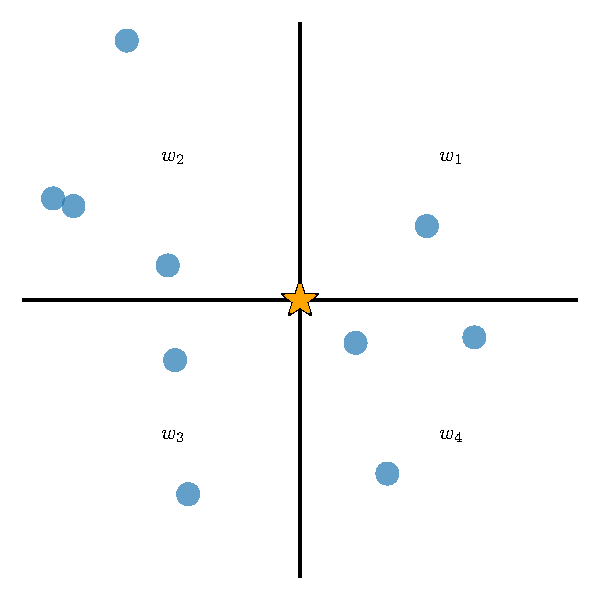
\includegraphics[width=.6\textwidth]{figures/RHD/flux_correction_method_plot.pdf}%
	\caption[Sketch of the weight correcting scheme for radiation injection]{
Sketch of the weight correcting scheme for radiation injection for a two-dimensional case. The
space
around a star which is surrounded by gas particles (blue circles) is divided into four quadrants.
The sum of all weights within a quadrant, $w_1$, $w_2$, $w_3$, $w_4$, is then used to improve the
isotropy of the injected energy and flux.
    }
	\label{fig:flux-injection-correction-method}
\end{figure}

A potential problem here is that unless the particle distribution is somewhat symmetric, the
resulting injected energy density (and flux) will not be isotropic, which is what stellar radiation
is typically assumed to be. So instead, we ``correct'' the weight $\psi_p$ in an attempt to improve
the isotropy of the deposited net energy and flux. We are limited in the manner we can compute the
correction term - we don't want the additional expense of a new star-particle interaction loop, nor
can we store all the neighbor data for every star individually in an attempt to determine isotropy.
So instead, we determine a correction term as follows.
For simplicity, let's consider the problem in 2D. We divide the space around a star into four
quadrants like in Figure~\ref{fig:flux-injection-correction-method}, and sum up the total weights
$\xi_s$ of the neighboring gas particles $g$ in each quadrant. This sum is denoted as $w_1$,
$w_2$, $w_3$, and $w_4$, as shown in Figure~\ref{fig:flux-injection-correction-method}. We now add
a correction factor $\mu_1$,  $\mu_2$,  $\mu_3$,  $\mu_4$ to each quadrant in an attempt to improve
the isotropy by applying two constraints:

\begin{enumerate}
    \item The total weight must remain constant:

\begin{equation}
\mu_1 w_1 + \mu_2 w_2 + \mu_3 w_3 + \mu_4 w_4 = w_1 + w_2 + w_3 + w_4
\end{equation}

    \item The modified weight of each quadrant should be equal, such that at least along these four
    directions, the injected energy and flux are isotropic:

\begin{equation}
\mu_1 w_1 = \mu_2 w_2 = \mu_3 w_3 = \mu_4 w_4
\end{equation}

\end{enumerate}

After some simple algebra, we arrive at

\begin{equation}
\mu_a = \frac{\oldsum_b w_b}{4 w_a} \label{eq:isotropy-correction-general}
\end{equation}

The extension to three dimensions is trivial: the factor 1/4 is just turned into 1/8, as we now
have octants instead of quadrants. The correction term~\ref{eq:isotropy-correction-general} needs a
small modification for cases where there is a octant which contains zero particles and hence zero
weight: Let $q_{nz}$ be the number of octants with non-zero weight, i.e. with non-zero particles
in them. Then

\begin{equation}
	\mu_a = \frac{\oldsum_b w_b}{q_{nz} w_a} \label{eq:isotropy-correction-with-zero}
\end{equation}


this ultimately gives us

\begin{align}
    \xi_s = \mu_a \ \psi(\x_{s} - \x_{g}, h(\x_{s}))
\end{align}

where $a$ is the octant in which the gas particle resides.


Since the weights in each octant are being collected for the anisotropy correction terms $\mu_a$,
we can in principle use any weight for particles instead of $\psi_i(\x)$ and use the total weight
to normalize the net injected energy and flux. Indeed, I tested particle weights $\xi_i \propto
r^{-\alpha}$ with $\alpha \in [0, 1, 2, 3]$ instead of the partition of unity $\psi_i(\x)$, but
none of these choices was able to out-perform the partitions of unity in terms of isotropy. The
reason is that the $\psi(\x)$ already contain information about neighboring particle positions
through the normalizations $\omega(\x)$ (eq.~\ref{eq:omega}). Additionally, the correction terms
$\mu_a$ can only improve isotropy, but not guarantee it, as they only take into account inequalities
between the octants around the star particle. For this reason, the choice of $\psi(\x)$ as the
individual weights is selected.



%
% Finally, as a sanity check, consider we have 1 star only, and sum the total energy injected into
% all gas particles.
%
% For any gas particle $p$, we have
%
% \begin{align}
%     E_i (\x = \x_{p}) = E_i(\x_{star}) \ \psi(\x_{star} - \x_{p}, h(\x_{star})) \ \mu_{a(p)}
% \end{align}
%
% with the definitions and constraints for the isotropy correction term $\mu_{a(p)}$:
%
% \begin{align}
%     w_{a(p)} &= \sum_{\mathrm{particles}\ p \in a} \psi(\x_{star} - \x_{p},  h(\x_{star}))\\
%     \sum_b w_b &= \sum_b w_b \mu_b\\
%     \sum_b w_b &= \sum_b \sum_{p\in b} \psi_p(h(\x_{star})) = \sum_{\text{all particles}\ p}
% \psi_p (h(\x_{star})) = 1
% \end{align}
%
% Then the sum over all particles is
%
% \begin{align}
%     \sum_p E_i (\x_{p}) &= \sum_p E_i(\x_{star}) \ \psi(\x_{star} - \x_{p}, h(\x_{star})) \
% \mu_{a(p)} \\
%         &= E_i(\x_{star}) \sum_p \ \psi(\x_{star} - \x_{p}, h(\x_{star})) \ \mu_{a(p)} \\
%         &= E_i(\x_{star}) \left( \sum_{p \in a} \ \psi_p \ \mu_{a} + \sum_{p \in b} \ \psi_p \
% \mu_{b} + ... \right)\\
%         &= E_i(\x_{star})  \sum_b \sum_{p \in b} \ \psi_p \ \mu_{b}\\
%         &= E_i(\x_{star})  \sum_b \mu_{b} \sum_{p \in b} \ \psi_p \\
%         &= E_i(\x_{star})  \sum_b \mu_{b} w_b \\
%         &= E_i(\x_{star})
% \end{align}
%
%
%
%
%






%------------------------------------------------------------------------------
\subsubsection{Injecting Photon Fluxes From Radiative Sources}
%------------------------------------------------------------------------------

A further topic with regards to injection of radiation from sources which requires a bit of
discussion is whether, and if so, in which manner to inject photon fluxes. For grid codes, the net
injected flux into a cell will automatically be zero since we assume that stars are points that
radiate isotropically, and the vector sum of an isotropic flux is zero. However for particle
codes, we don't have that luxury given automatically, as the total flux isn't injected into a
single cell, but into several particles. So as long as we can ensure that the vector sum of all
injected fluxes remains zero, we have some freedom to choose how (and how much) photon fluxes to
inject. However, if we inject the flux carelessly, we can end up with anisotropic fluxes.

% This is particularly important in the cases where we're especially interested in the effect of
% radiation pressure.

To inject fluxes, we could in principle use the same approach as for the energy density, and
inject the flux $\Fbf_{i,p,s}$ of photon group $i$ injected from star $s$ that we assign to a
particle $p$ according to

\begin{align}
	\Fbf_{i,p,s} &= \xi_s c E_{i,s} \mathbf{n}_{ps}  \\
    \mathbf{n}_{ps} &=  \frac{\x_p - \x_s}{|\x_p - \x_s|}
\end{align}

by making use of the energy density-flux relation for the optically thin limit $|\Fbf| = c E$, or
some other relation. What remains unclear is to determine (i) whether flux should be injected at
all, and (ii) if so, what energy density-flux relation to use. To this end, I tested three
different flux injection models:

\begin{itemize}
 \item The ``no flux injection'' model injects no radiation flux $\Fbf$. This corresponds to the
optically thick limit.
 \item The ``full flux injection'' model injects flux assuming an optically thin limit, i.e. $\Fbf
= c E$
 \item The ``modified flux injection'' model injects a linearly increasing amount of flux starting
with no flux and ending in the optically thin limit $\Fbf = c E$ at the distance $0.5H$, where $H$
is the maximal distance at which energy and flux is injected, i.e. the star's compact support
radius. For distances above $0.5H$, again the value of the optically thin limit is taken.
\end{itemize}

Note that (at least in ideal cases) the net injected flux, i.e. the vector sum of all injected
fluxes, still remains zero just as is the case for grid codes, but split among several gas
particles. The results are shown in Section~\ref{chap:results-injection}, where the ``no flux
injection'' model is shown to perform best.
















%-----------------------------------------------------------------------
\subsection{Second Step: Transport}\label{chap:transport-step}
%-----------------------------------------------------------------------

In this step, we solve
\begin{align}
    \DELDT{E_i} + \nabla \cdot \Fbf_i &= 0 \label{eq:homogenized-dEdt}\\
    \DELDT{\Fbf_i} + c^2 \nabla \cdot \mathds{P}_i &= 0 \label{eq:homogenized-dFdt}
\end{align}

They are both in the form of a hyperbolic conservation law
(\ref{eq:conservation-law-1D-introduction}), so we can use the finite volume particle method:

\begin{align}
	\deldt(\U_k V_k) + \sum\limits_{l} \mathcal F_{\alpha, kl} \mathcal{A}^\alpha_{kl} = 0
\label{eq:rt-meshless}
\end{align}

where $k$, $l$ are particle indices, $V_k$ the associated particle volumes
(eq.~\ref{eq:particle-volume}), $\mathcal{A}_{kl}$ the effective surfaces given
in eq.~\ref{eq:HopkinsAij}, and we have the state vector $\U$ and flux tensor $\F$

\begin{align}
	\U =
		\begin{pmatrix}
			E_i \\
			\Fbf_i
		\end{pmatrix}
	\quad , \quad
	\F =
		\begin{pmatrix}
			\Fbf_i \\
			c^2 \mathds{P}_i
		\end{pmatrix}
\end{align}

The total sum $\oldsum_l \F_{kl} A_{kl}$ for each particle $k$ is collected during a neighbor
interaction loop. Once the sum is accumulated, the final explicit update of the state is given by

\begin{align}
\U_k(t + \Delta t_k) =
	\U_k (t) - \frac{1}{V_k} \sum\limits_{l} \min\{\Delta t_k, \Delta t_l\}
    \F_{\alpha,kl} \mathcal{A}_{kl}^\alpha
\label{eq:transport-update-explicit}
\end{align}

To facilitate the individual time step sizes, the minimum between individual particle time steps
$\Delta t_k$ and $\Delta t_l$ is taken again, and the exchanged quantities between particles are
time integrated fluxes rather than just fluxes. The time integration needs to be the smaller of the
two time step sizes $\{\Delta t_k,\  \Delta t_l\}$ since if one particle has a smaller time step
size than the other, it also means that there will be several interactions between that particle
pair, each with the time step size of the smaller of the two. This ensures that the total exchange
of fluxes remains conservative, as the fluxes ``removed'' from particles $l$ remain exactly equal
to the fluxed ``added'' to particle $k$. If some neighboring particles $l$ have smaller time steps
than particle $k$, then the net sum of the fluxes is accumulated during the exchanges and applied
only at the point where particle $k$ is being updated again. More details on individual
timestepping is discussed in Section~\ref{chap:individual-timesteps}.



The number of neighbors each particle interacts with, or more precisely each particle's smoothing
length $h$, is the same as for hydrodynamics. This is necessary in order to be able to re-use all
quantities required to compute the effective surface terms \Aij and gradients of all radiation
fields. The precise number of neighbors is a free parameter, and is determined by specifying a
dimensionless parameter $\eta_{res}$ (see eq.~\ref{eq:number-of-neighbors}). The default choice is
$\eta_{res} = 1.2348$, which leads to approximately 48 neighbors for the cubic spline kernel
(eq.~\ref{eq:cubic-spline-kernel}). Note that the number of neighbors for star particles and for gas
particles can be specified using two independent parameters $\eta_{res}$, one for stars, and one for
the gas.

The time step size of the particles is computed in the same manner as we do it for hydrodynamics.
A ``cell size'' $\Delta x$ of a particle is estimated using

\begin{align}
    \Delta x \approx \left(\frac{V_i}{V_{S,\nu}} \right)^{1/\nu}
\end{align}

where $V_{S,\nu}$ is the volume of a $\nu$-dimensional unit sphere, i.e. $4/3 \pi$ in 3D. The signal
velocity in case of radiation is simply the speed of light $c$, which leads to the time step
estimate

\begin{align}
    \Delta t = C_{CFL} \frac{\Delta x}{c} \label{eq:rt-cfl}
\end{align}

A safe choice of $C_{CFL} \lesssim 0.6$ is recommended.



To get the inter-particle fluxes $\F_{kl}$, we also follow the scheme outlined by the finite volume
particle method in Section~\ref{chap:FVPM}. We use the ``Hopkins'' formulation of the method
(Section~\ref{chap:meshless-hopkins}), since the ``Ivanova'' version was shown to still have some
trouble in Section~\ref{chap:meshless-comparison}. Even though the radiative transfer is solved
assuming an Eulerian frame of reference, for which the ``Ivanova'' version is working adequately,
the ``Hopkins'' formulation seems like a safer and therefore better choice, at least for the time
being.

As it is done for the hydrodynamics in Section~\ref{chap:meshless-full}, we approximate the problem
by defining an ``interface'' at the position

\begin{equation}
	\mathbf{x}_{kl} = \mathbf{x}_k + \frac{h_k}{h_k + h_l} ( \mathbf{x}_l - \mathbf{x}_k )
\end{equation}

and extrapolate the value of the conserved variables at the position:

\begin{equation}
	\U_{k, l}(\mathbf{x} =
        \mathbf{x}_{kl}) \approx \U_{k, l} + \DELDX{ \U_{k, l}}\ (\mathbf{x}_{kl}
- \mathbf{x}_{k,l})
\end{equation}


such that the fluxes $\F_{kl}$ in the update formula~\ref{eq:rt-meshless} between particles is
estimated as the solution of the Riemann problem with ``left'' state $\U_k(\x_{kl})$ and ``right''
state $\U_l(\x_{kl})$

\begin{align}
    \F_{kl}
    = RP
    \left(\U_k + (\x_{k} - \x_{kl})_\alpha \DELDXALPHA{\U_k}, \
    \U_l + (\x_{l} - \x_{kl})_\alpha \DELDXALPHA{\U_l} \right) \label{eq:rt-riemann-problem}
\end{align}


The gradients $\DELDX{\U_{k,l}}$ are estimated again using the least-squares second order accurate
gradient expression given in eqn. \ref{eq:gradient}, for which a particle-particle interaction loop
is required. Since the RT is solved after the hydrodynamics and the particle positions haven't
changed since the last hydrodynamics drift, the particles' smoothing lengths are still accurate, and
we don't require an additional density loop for the radiative transfer. For that reason the gradient
particle loop constitutes the first particle interaction loop in the RT scheme.





%---------------------------------------------------
\subsubsection{Flux Limiters}
%---------------------------------------------------

The gradient extrapolation is equivalent from going from a piece-wise constant reconstruction of the radiation field to a piece-wise linear one, which makes the method second order accurate.
For each quantity $Q_{k,l} \in \U = (E_{k,l}, \Fbf_{k,l})^T$, we extrapolate the value at the
interface $\x_{kl}$ using the estimated gradient $dQ_{k,l}$. To prevent oscillations and
instabilities from occurring, we need to employ a flux limiter at this point, which effectively
reduces the gradient slopes $dQ_k$ and $dQ_l$ whenever necessary  (see
Section~\ref{chap:higher-order-schemes}). The limiters are implemented in such a way that they
return a factor $\alpha$, with which both slopes $dQ_k$ and $dQ_l$ are to be multiplied in order to
obtain the limited slopes, i.e:

\begin{align}
	\alpha &= \text{limiter}(dQ_k, dQ_l)\\
	dQ_{k, limited} &= \alpha\ dQ_k\\
	dQ_{l, limited} &= \alpha\ dQ_l
\end{align}

The two limiters that worked well in tests are the \emph{minmod limiter}

\begin{align}
% 	\alpha_{\text{minmod}}(dQ_k, dQ_l) =
% 		\begin{cases}
% 		\text{if } dQ_k \times dQ_l > 0:
% 			\begin{cases}
% 				\text{if } |dQ_k| < |dQ_l| :\quad &\alpha = dQ_k / dQ_l \\
% 				\text{else: } &\alpha = dQ_l / dQ_k\\
% 			\end{cases}\\
% 			\text{else: } \alpha = 0
% 		\end{cases}
    \alpha_{\text{minmod}}(dQ_k, dQ_l) =
    \begin{cases}
      dQ_k      & \text{ if } |dQ_k| < |dQ_l| \text{ and } dQ_k dQ_l > 0 \\
      dQ_l      & \text{ if } |dQ_k| > |dQ_l| \text{ and } dQ_k dQ_l > 0 \\
      0         & \text{ if }  dQ_k dQ_l \leq 0
    \end{cases} \label{eq:rt-minmod}
\end{align}

and the \emph{monotonized central difference (MC) limiter}:
\begin{align}
	r &= dQ_k / dQ_l \\
	\alpha_{\text{MC}}(r) &= \max \left\{ 0, \min\left[\frac{1 + r}{2}, 2, 2r \right] \right\}
	\label{eq:rt-MC}
\end{align}

The minmod limiter appears to be the most robust one with regards to ensuring stability for
radiative transfer, and for this reason is the recommended choice. The effects of the various
limiters on the transport of radiation will be shown in Section~\ref{chap:rt-riemann-limiters}.
Other possible choices are the \emph{superbee} limiter:

\begin{align}
	r &= dQ_k / dQ_l \\
	\alpha_{\text{superbee}}(r) &= \max \left\{0,  \min (1, 2r), \min(2, r) \right\}
	\label{eq:rt-superbee}
\end{align}


And the \emph{van Leer} limiter:

\begin{align}
	r &= dQ_k / dQ_l \\
	\alpha_{\text{vanLeer}}(r) &= \frac{r + |r|}{1 + |r|}
	\label{eq:rt-vanLeer}
\end{align}


While the slope and flux limiter combination described in \cite{hopkinsGIZMONewClass2015} for
hydrodynamics, whose full form is given in
eqns.~\ref{eq:face-limiter-first}-\ref{eq:face-limiter-last}, is a viable option, tests (shown in
Section~\ref{chap:rt-riemann-limiters}) have shown that it is more diffusive than the previously
described limiters for the application on radiation transport, and in some cases instabilities arise
that are seemingly connected to the first gradient limiting process. As such, I do not recommend to
use this sophisticated limiter in the context of RT. Note however that this limiter is used for
hydrodynamics, and that different flux limiting methods are used for hydrodynamics and radiative
transfer.


%
%Note to self:	We could try playing with $\gamma_1$ and $\gamma_2$ to minimize diffusion or other
%problems. We could even make it ``adaptive'', i.e. change them depending on whether we're in the
%optically thick or thin regime.
%
%
%
%Having computed the slope limited extrapolated conserved quantities $\U_{k}^{lim}$ and
%$\U_{l}^{lim}$, finally we compute the interparticle flux as
%
%\begin{equation}
%	\F_{kl} = \mathcal{RP}\left(\U_{k}^{lim}, \ \U_{l}^{lim}\right)
%\end{equation}
%
%
%where $\mathcal{RP}(...)$ is the Riemann problem with the index $k$ being the left side of the
%initial value problem and $l$ the right side.
%The Riemann problem can be solved using an approximate solver, which is discussed in the
%subsequent
%section.





%-------------------------------------------------------------------------------------------
\subsubsection{Riemann Solvers for the Moments of the RT equation}\label{chap:riemann-rt}
%-------------------------------------------------------------------------------------------

It remains to find a solution for the Riemann problem~\ref{eq:rt-riemann-problem} which gives us
the inter-particle (``inter-cell'') fluxes $\F_{kl}$.
To find $\F_{kl}$, we use the extrapolated and flux limited states $E_{k,l}$ and $\Fbf_{k,l}$ at the
interface position $\x_{kl}$ to compute the states and fluxes of the conservation law,
$\U_{k,l}(\x_{kl})$ and $\F_{k,l}(\x_{kl})$. The components of the vector valued photon flux density
$\Fbf_{k,l}$ are projected along the unit vector pointing from the particle towards the surface,
allowing us to treat each component individually as a one dimensional problem. We then adapt the
convention that particle $k$ is the left state of the Riemann problem, while particle $l$ is the
right state.

The \emph{Global Lax Friedrich (GLF)} Riemann solver \citep{ramses-rt13} then gives the
following solution for the flux $\F_{i+\half}$ between a cell $i$ and $i+1$:
\begin{equation}
	\F_{1/2}(\U_L, \U_R) =
		\frac{\F_{L} + \F_{R}}{2} -
		\frac{c}{2} \left(\U_R - \U_L \right) \label{eq:riemann-GLF}
\end{equation}

The GLF Riemann solver can be derived from the Lax-Friedrichs scheme, which for cells with sizes
$\Delta x$ takes the solution $\U_i^{n+1}$ to be the integral average of the solution
$\tilde{\U}(x, \Delta t/2)$ at the midpoint in time, $\Delta t/2$, of the Riemann problem which
uses the adjacent cells $i-1$ and $i+1$ as the left and right states, i.e.

\begin{align}
\U^{n+1}_i &=
    \frac{1}{\Delta x}
    \int_{-x_{i-\half \Delta x}}^{x_{i+\half \Delta x}} \tilde{\U}(x, \Delta t/2) \de x \\
\tilde{\U} &= RP(\U_{i-1}, \U_{i+1})
\end{align}

To proceed, we make use of the integral form of the conservation law
(eq.~\ref{eq:conservation-law-integral-form}) over the volume $[-\Delta x /2, \Delta x/2]$ and the
time interval $[0, \Delta t]$

\begin{align}
 \int\limits_{-\Delta x/2}^{\Delta x/2} \tilde{\U}(x, \Delta t/2) \de x  =
 \int\limits_{-\Delta x/2}^{\Delta x/2} \tilde{\U}(x, 0) \de x  +
 \int\limits_{0}^{\Delta t/2} \F(\tilde{\U}(-\Delta x /2, t)) \de t -
 \int\limits_{0}^{\Delta t/2} \F(\tilde{\U}(\Delta x/2, t)) \de t
\end{align}

The solution of the Riemann problem at $t = 0$ is simply the initial conditions, which in this
case is $\U_{i-1}$ on the left side, and $\U_{i+1}$ on the right side. The first integral on
the right hand side evaluates to

\begin{align}
\int\limits_{-\Delta x/2}^{\Delta x/2} \tilde{\U}(x, 0) \de x  =
\frac{\Delta x}{2} (\U_{i+1} + \U_{i-1})
\end{align}

The fluxes in the integrals are evaluated at the cell boundaries $-\Delta x/2$ and $\Delta x/2$.
Assuming an appropriate CFL condition is chosen, the resulting waves of the Riemann problem
situated at the cell center, which in this case is placed at $x = 0$, are not allowed to reach the
cell boundaries, i.e. travel a distance of $\Delta x/2$, by the time $\Delta t/2$. This means that
the states $\tilde{\U}$ at the cell boundaries $\pm \Delta x/2$ are constant in the time interval
$[0, \Delta t/2]$, and are also simply $\tilde{\U}(\pm\Delta x/2) = \U_{i\pm1}$. So the integrals
involving the fluxes evaluate to

\begin{align}
\int\limits_{0}^{\Delta t/2} \F(\tilde{\U}(\pm \Delta x /2, t)) \de t &=
    \int\limits_{0}^{\Delta t/2} \F(\U_{i\pm1}) \de t = \frac{\Delta t}{2} \F(\U_{i\pm1})
\end{align}

This leads to the scheme

\begin{align}
    \U_i^{n+1} = \frac{1}{2} (\U_{i-1} + \U_{i+1}) + \frac{1}{2} \frac{\Delta t}{\Delta x}
(\F^n_{i-1} - \F^n_{i+1})
\end{align}

which can be re-written as

\begin{align}
    \U_i^{n+1} =
        \U_i^n + \frac{\Delta t}{\Delta x} \left(\F_{i-\half}^{LF} - \F_{i+\half}^{LF} \right)
\end{align}

with the Lax-Friedrichs fluxes

\begin{align}
\F_{i+\half}^{LF} = \frac{1}{2} (\F^n_i + \F_{i+1}^n) + \frac{1}{2}\frac{\Delta x}{\Delta t} (
\U_i^n - \U_{i+1}) \label{eq:lax-friedrichs-flux}
\end{align}

By setting the Courant number to the maximally allowable value, $C_{cfl} = \frac{\Delta t}{\Delta x
c} = 1$, we can replace the term $\Delta t / \Delta x = c$ in eq.~\ref{eq:lax-friedrichs-flux},
and we obtain the GLF flux from eq.~\ref{eq:riemann-GLF}, where $c$ is the speed of light.




An alternative is the \emph{Harten - Lax - van Leer (HLL)} Riemann solver
(\cite{gonzalezHERACLESThreedimensionalRadiation2007}), which can be derived by assuming that the
solution of the Riemann problem consists of two discontinuous waves, and applying the
Rankine-Hugeniot jump conditions (eq.~\ref{eq:rankine-hugeniot}) across these waves. Like the
approximate HLLC solver for the Euler equations (discussed in Section~\ref{chap:riemann-hllc}), the
actual speed of the velocities needs to be estimated, for which the Eigenvalues of the conservation
law are used, as they describe the velocities of the characteristics (see
Chapter~\ref{chap:riemann}). Explicitly, the solver is given by

\begin{align}
	\F(\U_L, \U_R) &=
		\frac{ \lambda^{+} \F_{L} - \lambda^{-} \F_{R} +  \lambda^{+}
\lambda^{-} (\U_R - \U_L)}{ \lambda^{+} - \lambda^{-} }
\label{eq:riemann-HLL} \\
    \lambda^+ &= \max(0, \lambda_{max})\\
    \lambda^- &= \min(0, \lambda_{min})
\end{align}


Here, $\lambda^{max}$ and $\lambda^{min}$ are the minimum and the maximum of the Eigenvalues of the
Jacobian matrix $\frac{\del \F(\U)}{\del \U}$. It turns out that the Eigenvalues can be described
using only two parameters, the angle between the flux and the interaction interface, $\theta$, and
the reduced flux $\mathbf{f} = \Fbf / (cE)$. Rather then continuously computing them on-the-fly for
every interaction, they are tabulated\footnote{
A program to produce the tables of the Eigenvalues depending on $\theta$ and $\mathbf{f}$ is
provided on \url{https://github.com/SWIFTSIM/swiftsim-rt-tools}.
}
and interpolated. Note that the HLL solver predicts the same solution of the Riemann problem as the
GLF solver for $\lambda^{max} = c$, $\lambda^{min} = -c$ (compare eqs.~\ref{eq:riemann-GLF} and
\ref{eq:riemann-HLL}). The interest in the HLL solver is mainly because while it is more expensive
than the GLF solver, it was shown \citep{ramses-rt13, gonzalezHERACLESThreedimensionalRadiation2007}
to be less diffusive and is thus better suited to form shadows more correctly than the GLF solver.
The influence of the Riemann solvers are discussed in Sections~\ref{chap:results-transport} and
\ref{chap:Iliev3}.






%---------------------------------------------
\subsection{Third step: Thermochemistry}
%---------------------------------------------


In this final step, we solve for the interaction between photons and the gas. The equations to be
solved are:

\begin{align}
	\DELDT{E_i}  &=
		- \sum\limits_{j}^{\absorbers} n_j \sigma_{i j} c E_i + \dot E_i ^{rec}
\label{eq:thermochemistry-E} \\
	\DELDT{\Fbf_i} &=
		- \sum\limits_{j}^{\absorbers} n_j \sigma_{i j} c \Fbf_i \label{eq:thermochemistry-F}
\end{align}

The source term for recombination radiation, $\dot{E_i}^{rec}$, is added in
eq.~\ref{eq:thermochemistry-E} for completeness. In this work, the emission of recombination
radiation is neglected, and I use the approximate ``Case B recombination'' rates instead, which
assumes that all emitted recombination radiation is immediately re-absorbed by the gas, even in
optically thin regimes. However, once the emission of recombination radiation is treated explicitly
in the future, it will be added and solved for in this operator splitting step.

The actual thermochemistry is solved using the \grackle library
\citep{smithGrackleChemistryCooling2017}. This involves the evolution of the individual species
number densities, as well as the heating of the gas. The number densities of individual species
change over time due to processes like photo-ionization, collisional ionization, and recombinations.
These processes depend on the current gas temperature as well as the photo-heating and photo-ionizing rates which are determined by the present radiation field. Currently \GEARRT supports the ``6 species network'', composed of H$^0$, H$^+$, He$^0$, He$^+$, He$^{++}$, and $e^{-}$, provided by \grackle.

\grackle requires us to provide it with the (total) photo-heating rate $\mathcal{H} =
\oldsum_{i,j} \mathcal{H}_{ij}$ and the individual photo-ionization rates $\Gamma_{j} = \oldsum_i
\Gamma_{i,j}$ for each species $j$ and photon group $i$. It then solves the network of equations of
thermochemistry for the 6 species and evolves the internal energy of the gas over some time step
$\Delta t$. More precisely, \grackle takes into account the following interactions:

\begin{itemize}
 \item Collisional ionization of ionizing species H$^0$, He$^0$, and He$^+$
 \item Collisional excitation cooling of ionizing species H$^0$, He$^0$, and He$^+$
 \item Recombination of ions H$^+$, He$^+$, and He$^{++}$
 \item Bremsstrahlung cooling of all ionized species
 \item Compton cooling/heating off the Cosmic Microwave Background
 \item Photo-ionization and photo-heating.
\end{itemize}

While \grackle evolves the state of the gas, we need to take care of the removal of the absorbed
radiation energy over the thermochemistry time step manually.
We solve this again using a simple first order forward Euler integration:

\begin{align}
\frac{E_i (t + \Delta t) - E_i(t)}{\Delta t} =
    -\overline{\epsilon}_i N_i(t) c \ \sum_j \sigma_{i j} ^ N n_j
\end{align}

A minor complication is that the number density of the ionizing species $n_j$ is not constant over
the time step $\Delta t$, as we are currently in the process of ionizing the gas. This may lead to
scenarios where the absorption rate is overestimated by not accounting for the ionization during
the thermochemistry time step. To account for this effect, we take the average absorption rate over
the time step instead:


\begin{align}
    \frac{E_i (t + \Delta t) - E_i}{\Delta t}
        = -\overline{\epsilon}_i \ N_i(t) c \ \sum_j \sigma_{i j} ^ N  \
    \frac{n_j(t + \Delta t) + n_j(t)}{2}
\end{align}

The final equation used to remove absorbed photons from the radiation field is:

\begin{align}
E_i (t + \Delta t)
    &= E_i(t) - \overline{\epsilon}_i N_i(t) c \ \sum_j \sigma_{i j} ^ N  \
    \frac{n_j(t + \Delta t) + n_j(t)}{2} \ \Delta t \\
    &= E_i(t) \left(1 - c \ \sum_j \sigma_{i j} ^ N  \
    \frac{n_j(t + \Delta t) + n_j(t)}{2} \ \Delta t \right)
\end{align}

The same is applied to the photon fluxes:

\begin{align}
\Fbf_i (t + \Delta t)
    &= \Fbf_i(t) \left(1 - c \ \sum_j \sigma_{i j} ^ N  \
    \frac{n_j(t + \Delta t) + n_j(t)}{2} \ \Delta t \right)
\end{align}


















%------------------------------------------------------------------
\section{Dynamic Sub-Cycling}\label{chap:dynamic-sybcycling}
%------------------------------------------------------------------

Many radiation hydrodynamics solver codes \citep[e.g.][]{rosdahlSPHINXCosmologicalSimulations2018,
kannanAREPORTRadiationHydrodynamics2019} use a sub-cycling approach to solve the radiation transport
and thermochemistry using several dozens or hundreds of time steps over the duration of a single
hydrodynamics time step. This approach is motivated by the vastly different typical time step sizes
of hydrodynamics and radiation. The maximal permissible time step size is determined by their
respective CFL conditions (eq.~\ref{eq:rt-cfl} for radiation, and eq.~\ref{eq:meshless-cfl} for
hydrodynamics), which in turn each depend on the signal velocities of the respective conserved
quantities. Radiation, traveling at the speed of light of $\sim 3 \times 10^5$ km/s, usually has a
propagation velocity which is several orders of magnitude higher than fluid velocities, which in
the context of galaxies can reach orders of $\sim 10^2 - 10^3$ km/s, but is typically lower. This
also leads to the radiation time step sizes being similarly orders of magnitude smaller than
hydrodynamics time step sizes.

Enforcing the hydrodynamics and the radiative transfer to be solved using equal time step sizes
restricts the hydrodynamics time steps to much smaller sizes, which are not strictly necessary. So
the basic idea behind sub-cycling is, written in terms of the homogenized hydrodynamics operator $H$
and the source terms coming from radiation $S$, to modify the solution using equal time step sizes
$\Delta t$

\begin{align}
    \U(t + \Delta t) = S(\Delta t) \circ H(\Delta t)[\U(t)]
\end{align}

and to instead solve

\begin{align}
    \U(t + \Delta t) =
        S(\Delta t/n) \circ S(\Delta t/n) \circ ... \circ S(\Delta t/n) \circ H(\Delta t)[\U(t)]
\end{align}

where $n$ sub-cycles with time steps $\Delta t/n$ have been computed for a single homogenized
hydrodynamics operator $H$.


The sub-cycling approach allows us to save a tremendous workload. To motivate the possible benefits,
Figure~\ref{fig:taskplot-rt-marked} shows the same as in Figure~\ref{fig:taskplot}, tasks being
executed by 16 threads during one step solving radiation hydrodynamics with \swift, with the only
difference that the tasks have been given other colors: Orange blocks show tasks related to
radiative transfer only, blue tasks show the tasks related to hydrodynamics. Green tasks are tasks
related to the neighbor search, which can also be omitted during RT sub-cycles due to our choice to
treat radiation in a static frame of reference w.r.t. the simulation box (see
Section~\ref{chap:rt-numerics-outline}). Figure~\ref{fig:taskplot-rt-marked} shows that by skipping
unnecessary hydrodynamics updates by using sub-cycles, we could save roughly half the computational
expense per RT time step. The gains increase even further when other physics are involved.
Figure~\ref{fig:taskplot-rt-marked-gravity} shows the same radiation hydrodynamics problem being
solved with the addition of gravity. In this case, the fraction of the runtime occupied by RT tasks
is even smaller, meaning that by skipping needless updates of gravity and hydrodynamics (i.e.
forcibly reducing their time step sizes to match the RT time step sizes), we could save up a
significant amount of runtime. The actual reduction of runtime through the sub-cycling approach will
be de demonstrated in Section~\ref{chap:subcycling-results}.



\begin{figure}
 \centering
 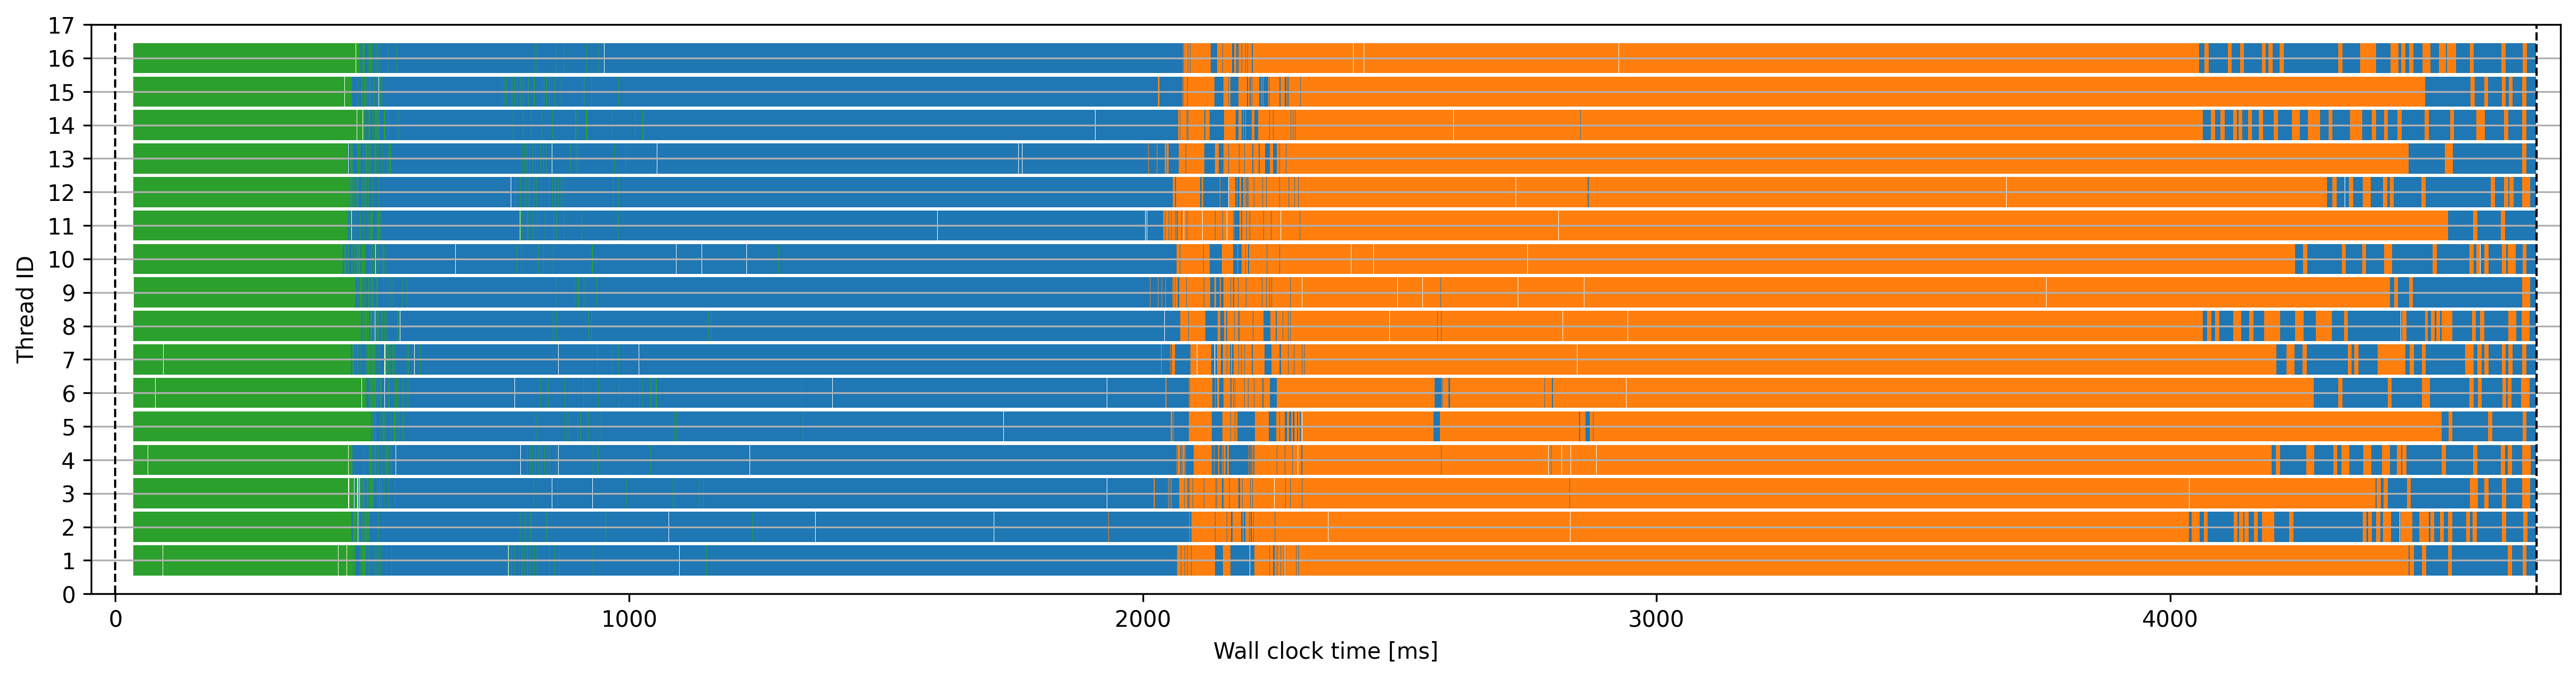
\includegraphics[width=\textwidth]{figures/RHD/taskplot-rt-colored.png}%
 \caption{
One time step of a simulation using \swift with 16 threads. This is the same plot as in
Figure~\ref{fig:taskplot}, but tasks have been colored in differently. Orange blocks show tasks
related to radiative transfer only, blue tasks show the tasks related to hydrodynamics. The
sub-cycling approach allows us to only solve the radiative transfer during each sub-cycle, saving
about half of the total runtime per sub-cycle through omission of the hydrodynamics. Green tasks
are tasks related to the neighbor search, which can also be omitted during RT sub-cycles due to our
choice to treat radiation in a static frame of reference w.r.t. the simulation box (see
Section~\ref{chap:rt-numerics-outline}).
 }
 \label{fig:taskplot-rt-marked}
\end{figure}


\begin{figure}
 \centering
 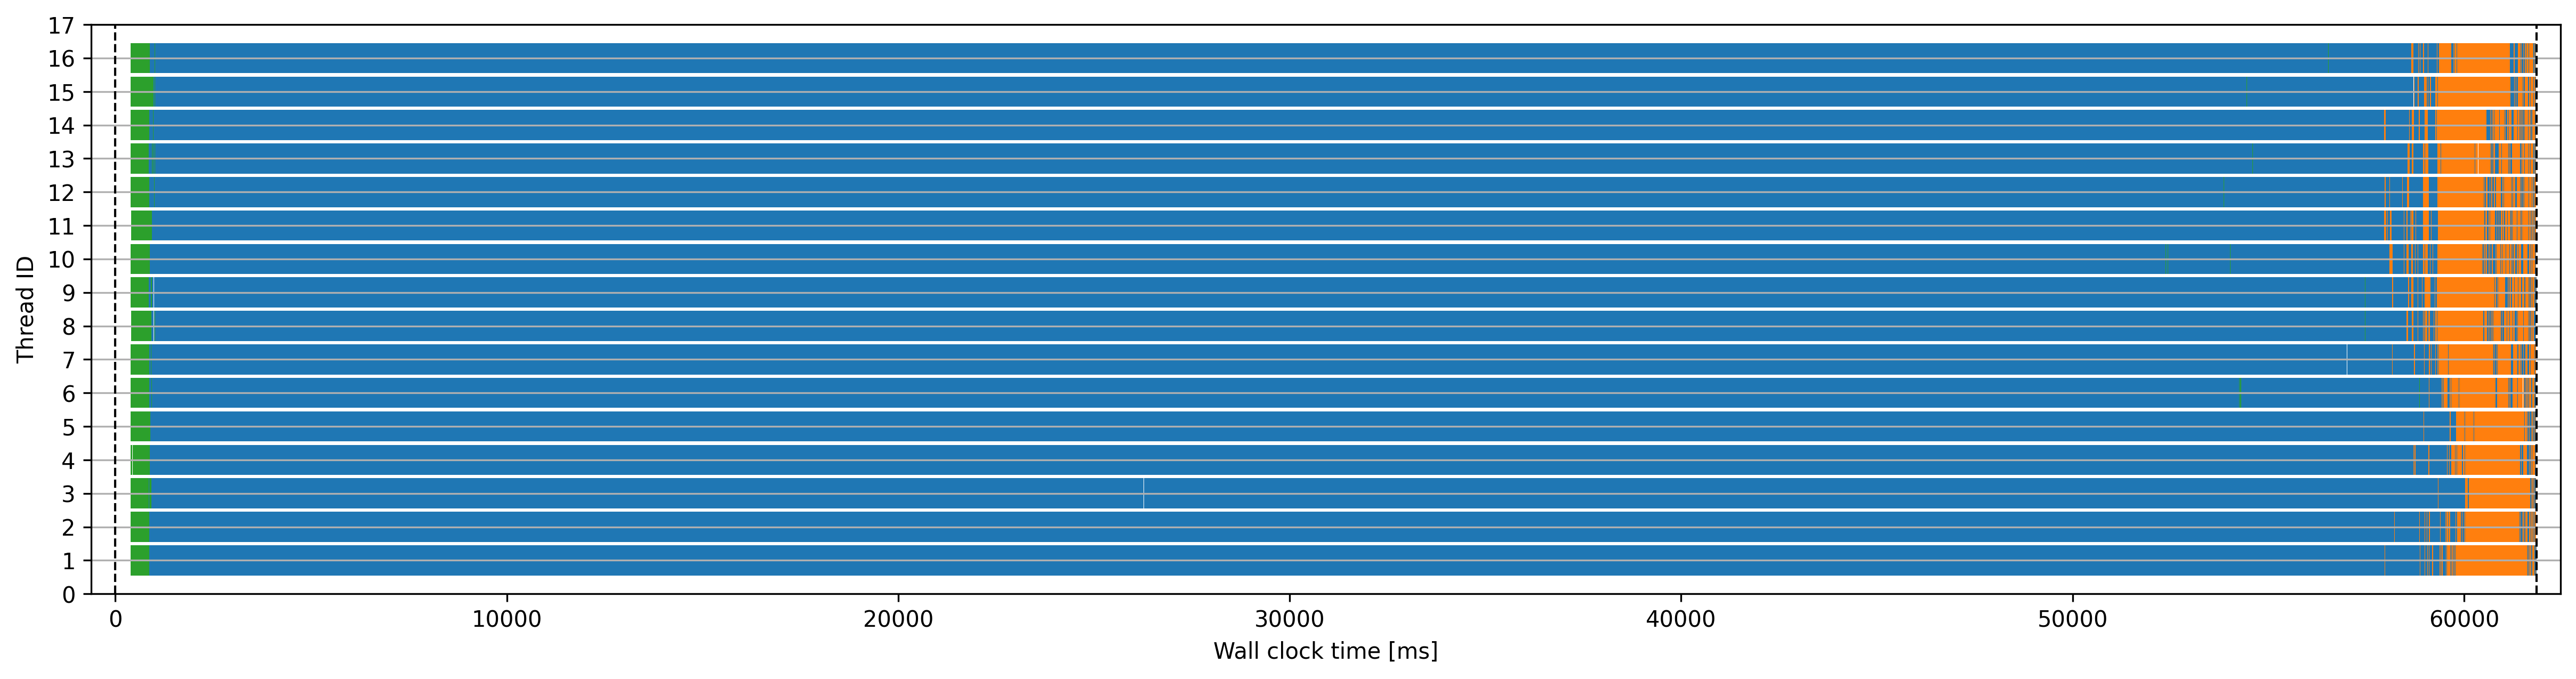
\includegraphics[width=\textwidth]{figures/RHD/taskplot-rt-colored-gravity.png}%
 \caption{
One time step of a simulation using \swift with 16 threads. This task plot includes (self-)gravity
in addition to radiation hydrodynamics. Orange blocks show tasks related to radiative transfer
only, blue tasks show the tasks related to hydrodynamics and gravity. Green tasks are tasks related
to the neighbor search, which can also be omitted during RT sub-cycles due to our choice to treat
radiation in a static frame of reference w.r.t. the simulation box (see
Section~\ref{chap:rt-numerics-outline}). The sub-cycling approach allows us to only solve the
radiative transfer during each sub-cycle, saving a huge fraction (the blue and green blocks) of the
total runtime per sub-cycle through omission of the hydrodynamics and gravity.
 }
 \label{fig:taskplot-rt-marked-gravity}
\end{figure}


\begin{figure}
 \centering
 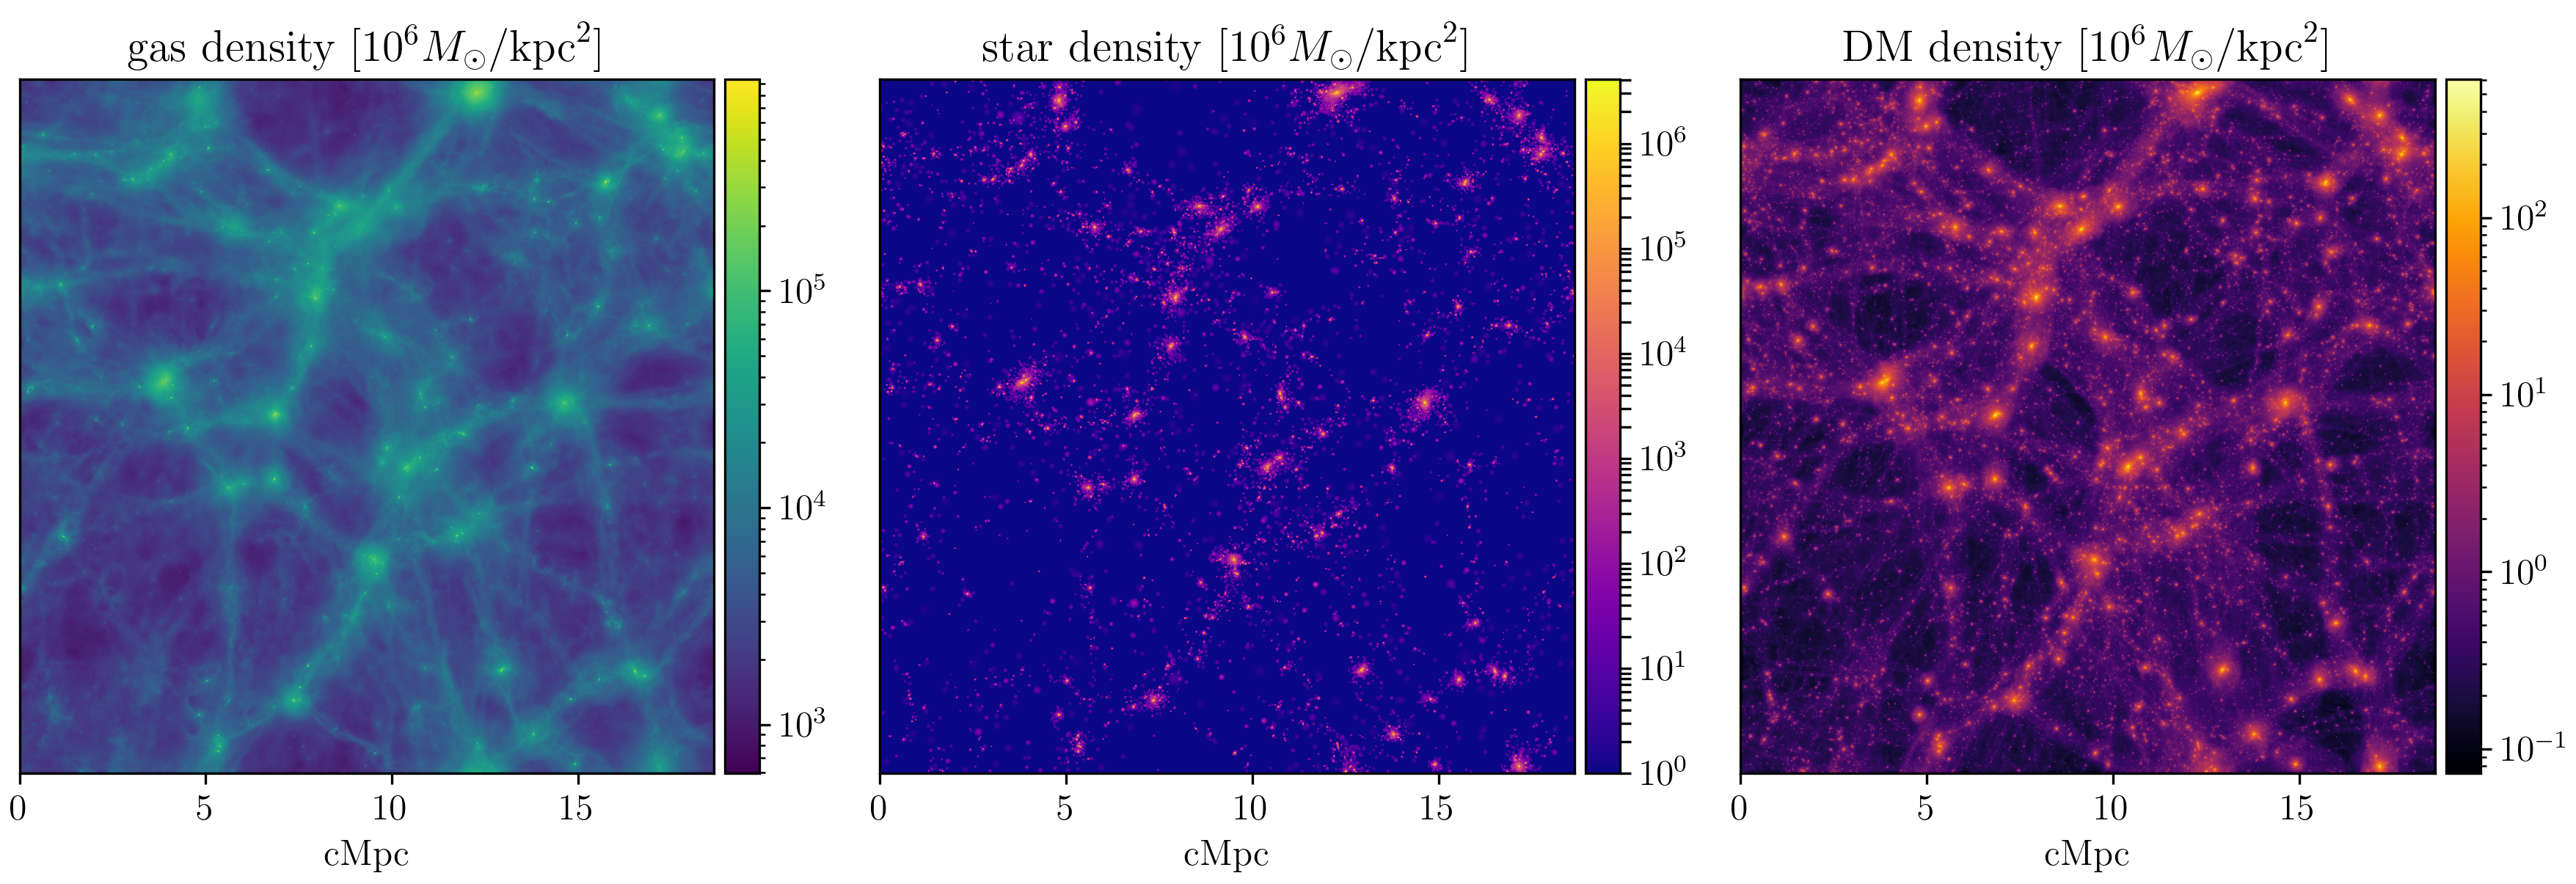
\includegraphics[width=\textwidth]{figures/RHD/EAGLE_25_ICs.png}%
 \caption{
Projections along the $z$-axis of the gas mass (left), the stellar mass (center), and dark matter
mass (right) of the simulation used to extract particles' radiation and hydrodynamics time bins
which are shown in Figure~\ref{fig:eagle-timebins-rt}. The simulation uses initial conditions
generated from the redshift $z = 0.1$  snapshots of the EAGLE suite of simulations
\citep{schayeEAGLEProjectSimulating2015}. It has a box size of $\sim 25$ co-moving Mpc and contains
$\sim 52 \times 10^6$ dark matter particles, $\sim 50 \times 10^6$ gas particles, and $\sim 2 \times
10^6$ star particles.\\
The initial conditions are publicly available via the \swift repository under
\url{https://github.com/SWIFTSIM/swiftsim}.
 }
 \label{fig:eagle-25}
\end{figure}



\begin{figure}
 \centering
 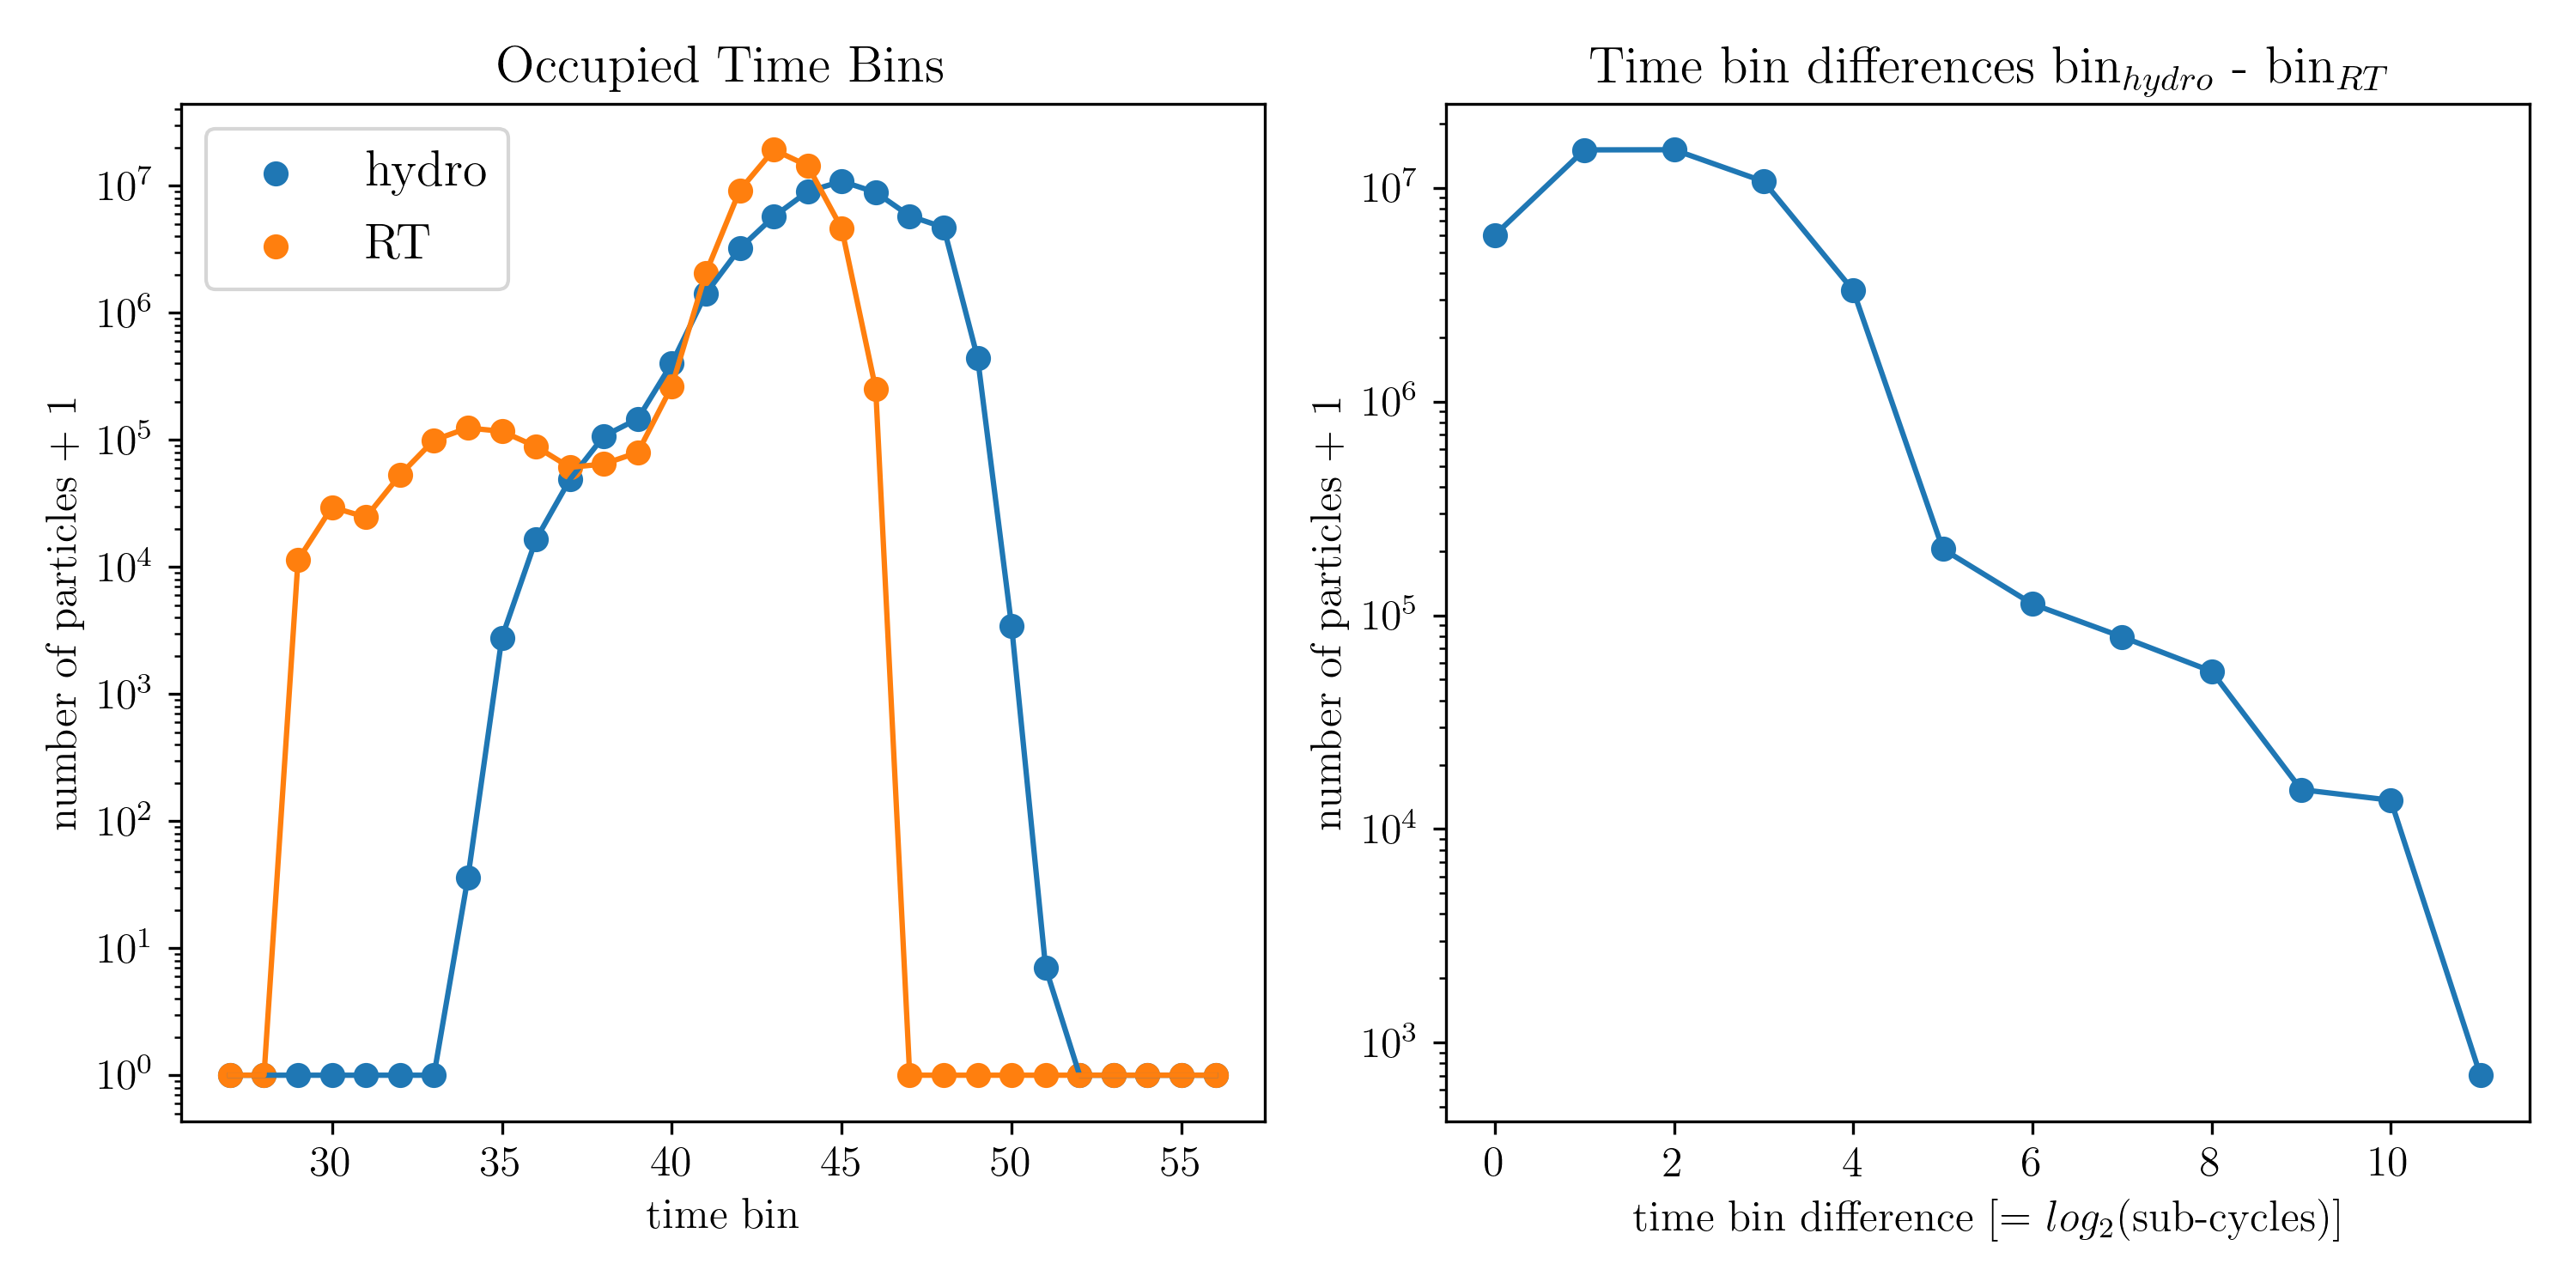
\includegraphics[width=\textwidth]{figures/RHD/subcycling_stats-64.png}%
 \caption{
\emph{Left}: The distribution of particle time bins for hydrodynamics and radiative transfer at a
single point in time in the simulation described in Figure~\ref{fig:eagle-25}. Particles with a
time bin $n + 1$ have a time step twice the size of particles with time bin $n$.\\
\emph{Right}: The distribution of time bin differences between the hydrodynamics time bin and the
RT time bin of each particle. This difference corresponds to the base 2 logarithm of the number of
sub-cycles each particle would perform. The upper limit of $2^{11} = 2048$ sub-cycles was imposed.
 }
 \label{fig:eagle-timebins-rt}
\end{figure}




An additional point that needs to be discussed with regards to the sub-cycling is how the number of
RT sub-cycles per hydrodynamics step is to be determined. On one hand, it is desirable to have as
many sub-cycles as possible to decrease the total runtime as far as possible. However, forcing
\GEARRT to perform \emph{too many} RT sub-cycles also introduces unnecessary work. For example, say
a particle has a hydrodynamics time step $\Delta t_h = 100$ in arbitrary units, while its RT time
step is $\Delta t_{rt} = 1$. Forcing \GEARRT to use 1000 sub-cycles leads to solving the radiative
transfer with unnecessarily reduced time steps of $\Delta t_{rt} = 0.1$. Clearly that's something
to be avoided. Instead, we allow each particle to set its number of sub-cycles individually
depending on its local conditions, and to change it dynamically after each completed hydrodynamics
step according to its own requirements. For example, a particle may perform 32 sub-cycles during one
hydrodynamics time step, during which the particle get heated and increases its internal energy,
which in turn decreases its hydrodynamics time step size due to the increased sound speed $c_s$
which enters the CFL condition~\ref{eq:meshless-cfl}. To continue the example, in the subsequent
hydrodynamics time step the particle may only require 16 or 8 RT sub-cycles. To further motivate
this approach, the time bins occupied for hydrodynamics and for radiative transfer extracted from a
cosmological simulation are shown in Figure~\ref{fig:eagle-timebins-rt}. (Details on the simulation
are given in the caption of Figure~\ref{fig:eagle-25}.) In order to facilitate a synchronous
integration in time alongside individual particle time step sizes, the time steps are histogrammed
into power-of-two multiples of some minimal system time step size, i.e. $\Delta t_i = 2^n t_{min}$,
where $n$ is usually referred to as the ``time bin'' of the particle (as described in
Section~\ref{chap:individual-timesteps}). Figure~\ref{fig:eagle-timebins-rt} illustrates that there
is a wide range of time step sizes, or rather time bins, for both hydrodynamics and radiative
transfer occurring. Figure~\ref{fig:eagle-timebins-rt} furthermore shows that there is a wide range of
RT sub-cycles occurring, including the maximal permitted value in that example of $2^{11} = 2048$,
which corresponds to a time bin difference of $11$.\footnote{
Arguably a maximal permitted number of RT sub-cycles of $2048$ is a bit unreasonably high. It was
used in Figure~\ref{fig:eagle-timebins-rt} for illustrative purposes. The maximal number of
sub-cycles is a free parameter, and should be determined depending on the actual use case at hand.
It should however probably not exceed 512 or 1024.
}
Notably, there is also a significant amount of particles with equal RT and hydrodynamics time bins,
validating the approach to let particles decide for themselves how many sub-cycles they require,
rather than enforcing a fixed number of sub-cycles for all particles. It should however be noted
that a time step limiter is being employed as well. Following the findings of
\citet{saitohNecessaryConditionIndividual2009} and \citet{durierImplementationFeedbackSmoothed2012},
any two particles that interact with each other are enforced to have a maximal time step difference
of a factor of 4 (or equivalently, a difference in time bins of 2) in order to preserve energy
conservation. This limiter is applied to both the hydrodynamics and to the radiative transfer
solvers individually.

While the fundamental approach of sub-cycling the radiative transfer is fairly straightforward, its
implementation while accounting for individual particle time step sizes and task-based parallelism
used in \swift were a considerable challenge. The details of the implementation are presented in
Section~\ref{chap:subcycling}.











%---------------------------------------------
\section{Additional Topics}
%---------------------------------------------


%---------------------------------------------
\subsection{Dealing With Particle Drifts}\label{chap:rt-drift}
%---------------------------------------------

As outlined in Section~\ref{chap:rt-numerics-outline}, while we assume particles are static w.r.t.
the simulated volume in the context of RT, they are drifted for the purposes of hydrodynamics. As a
consequence, we need to make corrections to the radiation fields when a particle is drifted for
hydrodynamics purposes. We do that by simply extrapolating the particle value at the new point given
its current state and the gradients $\nabla \U$ we obtained using the general gradient expression
given in eq~\ref{eq:gradient}. Explicitly, for a particle $i$ and for each component of the
radiation state vector $\U^k$, we first obtain the drift distance over the time $\Delta t_{i,
drift}$ as

\begin{align}
\Delta \x_{i,\text{drift}} &= \V_{i} \Delta t_{i,\text{drift}}
\end{align}

where $\V_i$ is the particle velocity. We then obtain the value corrected at the drifted
location

\begin{align}
\U_{i}^k (\x + \Delta \x_{\text{drift}}) \approx \U_{i}^k (\x) + \nabla \U_{i}^k (\x) \cdot \Delta
x_{i,\nu,\text{drift}}
\end{align}

A caveat for these corrections is that they are  no longer strictly conservative for obvious
reasons: Firstly, we use gradients to extrapolate what the radiation field values at the drifted
position should be. Secondly, the gradients themselves are only approximate and $\mathcal{O}(h^2)$
accurate. Thirdly, there are no further mechanisms to ensure that the resulting radiation field
quantities are actually conserved in total. However, the error introduced is acceptably small, as
will be shown in Section~\ref{chap:validation-drift-corrections}, where the application of these
corrections is validated.












%---------------------------------------------
% \subsection{Cosmology}
%---------------------------------------------
% \todo{all of this}





%---------------------------------------------
\subsection{Reducing The Speed of Light}
%---------------------------------------------


A huge challenge related to radiative transfer is the very high speed of light compared to the
fluid velocities. Since the signal velocity determines the maximal time step size, the speed of
light leads to minute time step sizes for the radiative transfer, several orders of magnitude
smaller than those for the hydrodynamics. Indeed this discrepancy is the main motivation to solve
radiative transfer with in a sub-cycling manner, which is discussed in
Section~\ref{chap:subcycling}.

In an attempt to reduce the computational expense associated with these tiny time step sizes,
\cite{ramses-rt13} employ the Reduced Speed of Light Approximation (RSLA), which was introduced by
\cite{gnedinMultidimensionalCosmologicalRadiative2001}. I also adapt the RSLA with \GEARRT. The
approach consists of globally reducing the speed of light everywhere by some factor $f_c$, i.e.
replace the speed of light $c$ in all equations involved with radiative transfer by

\begin{align}
    \tilde{c} = f_c c
\end{align}

Naturally, this means that the radiation will propagate (much) slower than it actually should.
However, that does not necessarily mean that the propagation of ionization fronts will be slowed
down as well. \cite{gnedinMultidimensionalCosmologicalRadiative2001} argue that as long as the
reduced speed of light remains much higher than the gas velocity, the Newtonian limit (in which the
speed of light is infinite) is maintained, and the evolution of ionized fronts is not hindered.
\cite{ramses-rt13} provide a framework to estimate the smallest permissible $f_c$ based on the
light crossing time in spherical ionized regions around a single ionizing source, also known as
``Str\"omgren spheres''. For example, they estimate that for the interstellar medium modeled with
a number density of $n = 10^{-1}$ cm$^-3$ and an ionizing source of $2 \times 10^{50}$ ionizing
photons per second, $f_c$ may be $\sim 10^{-2}$.

Note that the reduced speed of light $\tilde{c}$ is not only used in the photon transport, but also
to compute the photo-heating and photo-ionization rates (eq.~\ref{eq:photoheating-group} and
\ref{eq:photoionization-group}). This can be understood when considering the photo-heating and
photo-ionizations as binary collisions between photons and photo-absorbing particles, which are
treated as targets in this scenario. Now consider a photon packet, like a top hat function,
traveling at the reduced speed $\tilde{c}$. In the binary collision scenario, the photons are
projectiles being propelled at the targets with their velocity $\tilde{c}$, and as discussed in
Section~\ref{chap:coupling-to-hydrodynamics}, the interaction rates are directly proportional to
that velocity. For $\tilde{c} < c$, this means that the interaction rates, and thus the
photo-ionization rates, will also be decreased. However, since the photon packet travels at a
reduced
speed, it will spend a longer time passing through the location of the targets, which in turn again
increases the total number of photo-ionization events. So keeping the speed of light at its actual
physical value in the interaction rates while decreasing it for the photon transport would lead to
an over-ionization over time, which is what \cite{ocvirkImpactReducedSpeed2019} have also found.












%---------------------------------------------
\subsection{Ion Mass Fluxes}
%---------------------------------------------

Hydrodynamics with Finite Volume Particle Methods exchange mass fluxes $\Delta m$ between particles.
This means that we need to pay attention to the individual ionizing and ionized species' mass
fractions being exchanged. The mass of each individual species being exchanged needs to be traced
individually, and depending on the direction: If a particle loses mass, then it loses mass and
species mass fractions according to its own mass fractions. If it gains mass during an exchange,
then it gains species mass fractions according to the interaction partner's mass fractions.

The usual convention for a mass flux between particles ``$i$'' and ``$j$'' is to treat $i$ as the
``left'' particle and $j$ as the ``right'' particle in an analogy to cells. Let $X_k$ denote the
mass fraction of each species $k$. During each \emph{hydrodynamics} flux exchange, for each species
$k$ the total mass flux $\Delta x_{i,k}$ is being accumulated:

\begin{align}
\Delta x_{i,k} &= \sum_j \Delta m_{ij} X_{ij,k}\\
\text{where }\quad X_{ij,k} &=
	\begin{cases}
		X_{i,k} \quad \text{ if } \quad \frac{\Delta m_{ij}}{\Delta t} > 0 \\
		X_{j,k} \quad \text{ if } \quad \frac{\Delta m_{ij}}{\Delta t} < 0
	\end{cases}
\end{align}

The masses which particles carry are updated during the kick operation, during which the individual
species' masses $x_{i,k}$ are also evolved. For a particle $i$ with mass $m_i$, the masses of
individual species at the beginning of a step are given by:

\begin{align}
    x_{i,k}^{t} &= m_i X_{i,k}^{t}
\end{align}

During the kick operation, they get updated as follows:

\begin{align}
    x_{i,k}^{t + \Delta t} &= x_{i,k}^{t} + \Delta x_{i,k}
\end{align}

Finally, after the update, the new mass fractions of the species can be obtained using

\begin{align}
X_{i,k}^{t + \Delta t} &= \frac{x_{i,k}^{t + \Delta t}}{\sum_k x_{i,k}^{t + \Delta t}}
\end{align}










%-------------------------------------------------------------------------
\subsection{Creating Collisional Ionization Equilibrium Initial Conditions}
%-------------------------------------------------------------------------

At the beginning of a simulation, \GEARRT offers the possibility to generate the ionization mass
fractions of the gas particles assuming the gas is in collisional ionization equilibrium, composed
of hydrogen and helium, and that there is no radiation present. In order to determine the
ionization mass fractions of all species (H$^0$, H$^+$, He$^0$, He$^+$, He$^{++}$) for a given
specific internal energy $u$, an iterative procedure needs to be applied because the gas variables
are interconnected in a circular manner. To explain this circular dependence, we make use of the
(unitless) mean molecular weight $\mu$, which is commonly used to express the average particle mass
$\overline{m}$ of a gas:

\begin{align}
    \overline{m} = \mu m_u
\end{align}

where $m_u$ is the atomic mass unit. To begin, we note that the ionization state of the gas
influences the mean molecular weight $\mu$. Consider a medium with $j$ different elements of atomic
mass $A_j$ with a mass fraction $X_j$ and a number of free electrons $E_j$. Then the number density
of the gas is given by

\begin{align}
n = \frac{\rho}{\mu m_u}
    = \sum_j
    \underbrace{\rho X_j}_{\text{density fraction of species } j} \times
    \underbrace{\frac{1}{A_j m_u}}_{\text{mass per particle of species}} \times \underbrace{(1 +
    E_j)}_{\text{number of particles per species}} \label{eq:number-density-MMW}
\end{align}

where we neglect the mass contribution of electrons. In the case for hydrogen and helium, the values
of $A_j$ and $E_j$ are shown in Table \ref{tab:mass-and-electron-numbers}.
Eq.~\ref{eq:number-density-MMW} simplifies to

\begin{align}
\frac{1}{\mu} = \sum_j \frac{X_j}{A_j} (1 + E_j)
\end{align}

Specifically, ionization changes the mass fractions $X_j$ of the species, and therefore also the
mean molecular weight $\mu$. In turn, the mean molecular weight determines the gas temperature at a
given specific internal energy. Using the equation of state for ideal gases using the pressure $p$,

\begin{align}
    p = n k T = \frac{\rho}{\mu m_u} k T
\end{align}

and the expression for the specific internal energy  $u$,

\begin{align}
    u = \frac{1}{\gamma - 1} \frac{p}{\rho}
\end{align}

the gas temperature $T$ = $T(u, \mu)$ is given by

\begin{align}
    T = u (\gamma - 1) \mu \frac{m_u}{k}
\end{align}

Lastly, the gas temperature determines the collisional ionization and recombination rates, which
need to be balanced out by the correct number density of the individual species in order to be in
ionization equilibrium, i.e. at a state where the ionization and recombination rates exactly cancel
each other out. We take the ionization and recombination rates from
\citet{katzCosmologicalSimulationsTreeSPH1996}, which are given in Table
\ref{tab:coll-ion-rates-katz}. For a gas with density $\rho$, hydrogen mass fraction $X_H$ and
helium mass fraction $X_{He} = 1 - X_H$, the total number densities of all hydrogen and helium
species are

\begin{align}
    n_H &= X_H \frac{\rho}{m_u} \\
    n_{He} &= X_{He}  \frac{\rho}{4 m_u}
\end{align}

and in equilibrium, the number densities of the individual species are given by

\begin{align}
n_{H^0} &= n_H \frac{A_{H^+}}{A_{H^+} + \Gamma_{H^0}} \\
n_{H^+} &= n_H - n_{H^0} \\
n_{He^+} &= n_{He} \frac{1}{1 + (A_{He^+} + A_d) / \Gamma_{He^0} + \Gamma_{He^+} / A_{He^{++}}} \\
n_{He^0} &= n_{He^+} \frac{A_{He^+} + A_d}{\Gamma_{He^0}} \\
n_{He^{++}} &= n_{He^+} \frac{\Gamma_{He^+}}{A_{He^+}}
\end{align}

To summarize, the tricky bit here is that the number densities determine the mean molecular weight,
the mean molecular weight determines the temperature of the gas for a given density and specific
internal energy, while the temperature determines the number densities of the species through the
ionization rates. To find the correct mass fractions, the iterative Newton-Raphson root finding
method is used. Specifically, using some initial guesses for temperature and mean molecular
weights, $T_{guess}$ and $\mu_{guess}$, in each iteration step we determine the resulting specific
internal energy

\begin{align}
u_{guess} = k T_{guess} / (\gamma - 1) / (\mu_{guess} m_u)
\end{align}

The function whose root we're looking for is

\begin{align}
    f(T) = u - u_{guess}(T)  = 0
\end{align}

which has the derivative

\begin{align}
\frac{\del f}{\del T} =
    - \frac{\del u}{\del T} (T = T_{guess}) =
    \frac{k}{(\gamma - 1) / (\mu_{guess} m_u )}
\end{align}

The specific internal energy of the gas $u$ is fixed and provided by the initial conditions. We now
look for the $T$ at which $f(T) = 0$. The Newton-Raphson method prescribes to find the $n+1$th
$T_{guess}$ using

\begin{align}
    T_{n+1} = T_n + \frac{f(T_n)}{\frac{\del f}{\del T}(T_n)} \ .
\end{align}

During each iteration, the new mass fractions and the resulting mean molecular weight given the
latest guess for the temperature are computed. At the start, the first guess for the temperature
$T_{guess}$ is computed assuming a fully neutral gas. Should that gas temperature be above $10^5$
K, the first guess is changed to a fully ionized gas. The iteration is concluded once $f(T) \leq
\epsilon = 10^{-4}$. The results \GEARRT provides for a wide range of temperatures is shown in
Figure~\ref{fig:ionization-equilibrium}.


\begin{figure}
 \centering
 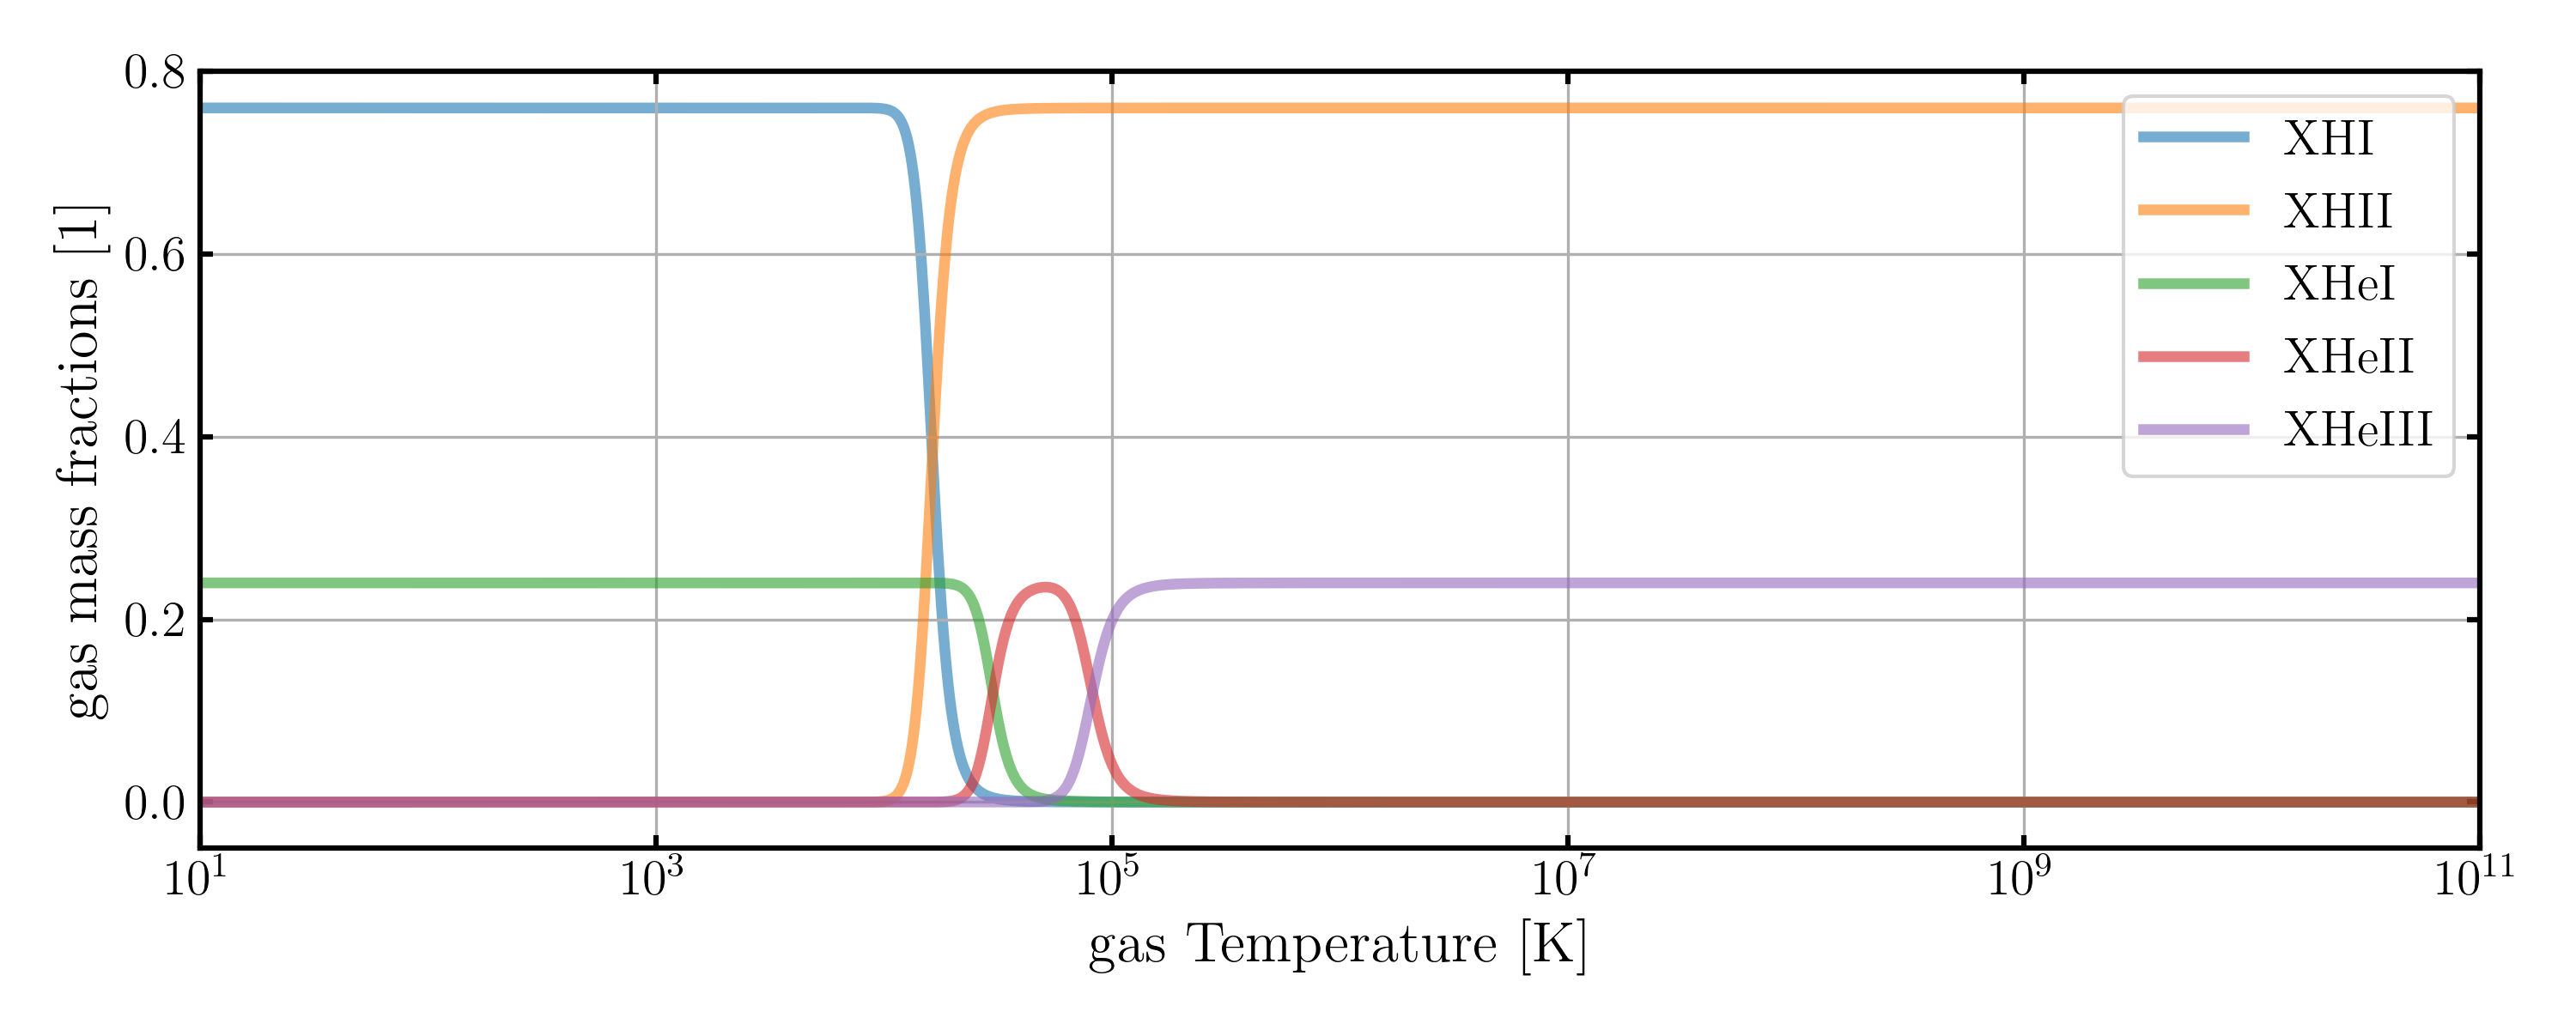
\includegraphics[width=.8\textwidth]{figures/RHD/ionization_equilibrium.png}
 \caption{
Mass fractions of hydrogen and helium ion species in collisional ionization equilibrium  as
computed by \GEARRT for a wide range of temperatures $T$, corresponding to specific internal
energies of the gas between $10^9$ erg/g and $10^{20}$ erg/g, specified by the initial conditions.
The initial composition of the gas consists of 76\% hydrogen and 24\% helium by
mass.
 }
 \label{fig:ionization-equilibrium}
\end{figure}

\begin{table}
\begin{center}
\begin{tabular}{lll}
\hline\\
$A_{H^+}         $ & 
    $8.4 \times 10^{-11} T^{-1/2} T_3^{-0.2} (1 + T_6^{0.7})^{-1}$ & 
    RR for H$^{+}$ 
\\[.5em]
$A_{d}           $ &
    $1.5 \times 10^{-10} T^{-0.6353}$    & 
    dielectronic RR for He$^{+}$ 
\\[.5em]
$A_{He^+}        $ & 
    $1.9 \times 10^{-3} T^{-1.5} \mathrm{e}^{-470000/T} (1 + 0.3 \mathrm{e}^{-94000/T})$    & 
    RR for He$^{+}$
\\[.5em]
$A_{He^{++}}     $ & 
    $3.36 \times 10^{-10} T^{-1/2} T_3^{-0.2} (1 + T_6^{0.7})^{-1}$    & 
    RR for He$^{++}$
\\[.5em]
\hline\\
$\Gamma_{H^{0}}  $ & 
    $5.85 \times 10^{-11} T^{1/2} \mathrm{e}^{-157809.1/T} ( 1 + T_5^{1/2})^{-1}$& 
    CIR for H$^{0}$
\\[.5em]
$\Gamma_{He^{0}} $ & 
    $2.38 \times 10^{-11} T^{1/2} \mathrm{e}^{-285335.4.1/T} ( 1 + T_5^{1/2})^{-1}$& 
    CIR for He$^{0}$
\\[.5em]
$\Gamma_{He^{+}} $ & 
    $5.68 \times 10^{-12} T^{1/2} \mathrm{e}^{-631515/T} ( 1 + T_5^{1/2})^{-1}$& 
    CIR for He$^{+}$
\\[.5em]
\hline
\end{tabular}
\end{center}
\caption{Temperature ($T$) dependent recombination rates (RR) and collisional ionization rates 
(CIR) for Hydrogen and Helium species, adapted from \citet{katzCosmologicalSimulationsTreeSPH1996}. 
All rates are in units of cm$^3$ s$^{-1}$. $T_n$ is shorthand for $T / 10^n$K.}
\label{tab:coll-ion-rates-katz}
\end{table}



\begin{table}
\begin{center}
\begin{tabular}{l|ll}
species  & $A$ & $E$ \\
\hline
H$^0$    & 1 & 0 \\
H$^+$    & 1 & 1 \\
He$^0$   & 4 & 0 \\
He$^+$   & 4 & 1 \\
He$^{++}$  & 4 & 2 \\
\end{tabular}
\end{center}
\caption{Atomic mass numbers $A$ and free electron numbers $E$ for ionization species of Hydrogen 
and Helium.}
\label{tab:mass-and-electron-numbers}
\end{table}











%------------------------------------------------------------
\section{Implementation in SWIFT}\label{chap:rt-implementation}
%------------------------------------------------------------

%------------------------------------------------------------
\subsection{Task Dependency Graph for Radiative Transfer}
%------------------------------------------------------------

Just as for the hydrodynamics in Chapter~\ref{chap:meshless-implementation}, the task-based
parallelism used by \swift requires the manual definition of the individual tasks and dependencies
that solve the numerical scheme. In this section, we do this for radiative transfer with \GEARRT.

The tasks required for RT will be added to the already existing tasks which are required for the
hydrodynamics. A simplified sketch is shown in Figure~\ref{fig:RTtaskplot-simplified}. The full
task dependency graph for hydrodynamics is shown in Figure~\ref{fig:dependency-graph-hydro}. As
mentioned before, the radiative transfer will take place \emph{after} the hydrodynamics have been
solved, or explicitly after the ``\lingo{kick2}'' task in Figure~\ref{fig:dependency-graph-hydro}.

The first step of RT, namely the injection of radiation energy density from stellar sources into
particles, requires two interaction loops for star particles. The first loop constitutes a neighbor
search for stars, during which the stars' smoothing lengths and neighbor lists of gas particles are
established. We make use of this first loop to accumulate the octant weights $w_a$ (which are
discussed in Section~\ref{chap:injection-step}) in order to be able to compute the weight
corrections $\mu_a$ (eq.~\ref{eq:isotropy-correction-with-zero}) during the second star-gas particle
interaction loop. The actual injection of energy density into particles then occurs during this
second star-gas particle interaction loop.

Other stellar feedback processes in \swift require the same two interaction loops for the exactly
same reasons. As the injection of radiation energy density is in principle independent from these
feedback processes, we can conveniently re-use these tasks, i.e. add the injection of radiation to
them. Additionally, the \lingo{star ghost} task, which is required between the two interaction
loops for stars for the same reasons it is necessary after the neighbor search (``\lingo{density}'')
loop for hydrodynamics, can be used to compute the amount of energy each star needs to inject this
step based on their current luminosity and time step sizes.

After the injection through the star-gas particle interaction loops, a first RT ghost task
(``\lingo{rt\_ghost1}'') is added to finish any necessary work after the accumulation of injected
radiation, and to collect all dependencies before proceeding further down the dependency graph.
Since not all gas particles need to have a neighboring star particle, some gas particles may not
undergo the injection process. For this reason, an additional dependency from \lingo{kick2} to the
\lingo{rt\_ghost1} task is necessary (see Figure~\ref{fig:RTtaskplot-simplified}).

The next step in the RT scheme consists of the photon transport step, which needs to be done in two
parts. First, a gas-gas particle interaction loop is necessary to determine the gradients of the
radiation quantities, which are required for the flux exchanges. The flux exchanges are then
performed in a second gas-gas particle interaction loop, named the ``\lingo{transport}'' loop.
Between the \lingo{gradient} and the \lingo{transport} loop, a second ghost task,
``\lingo{rt\_ghost2}'', is required to finish the gradient computations after the accumulation of
sums in the \lingo{gradient} loop is completed.

The ``\lingo{thermochemistry}'' task solves the final step in the RT scheme, which consists of the
actual thermochemistry. All the required work is on individual particles, which can be modeled as a
\lingo{plain} type task.

Figure~\ref{fig:RTtaskplot-nosubcycling} shows the full task dependency graph for radiation
hydrodynamics with \GEARRT and \swift. The interaction loops have been expanded to depict all four
types of \lingo{interaction} type tasks, which are the \lingo{self}, \lingo{sub\_self},
\lingo{pair}, and \lingo{sub\_pair} tasks, for both the star interaction tasks
(``\lingo{stars\_density}'' and ``\lingo{stars\_feedback}'', in orange) and the RT interaction tasks
(``\lingo{rt\_gradient}'' and ``\lingo{rt\_transport}'', in green). Additionally, the MPI
communication tasks have been added. Just as was the case for hydrodynamics, the current state of
the particles needs to be sent and received before each interaction loop, using the respective
``\lingo{send\_rt\_gradient}'', ``\lingo{recv\_rt\_gradient}'' and ``\lingo{send\_rt\_transport}'',
``\lingo{recv\_rt\_transport}'' tasks. Dependencies between the sending tasks and the receiving
tasks are necessary, respectively, in order to assure the order of messages arriving being correct,
and to prevent race conditions since the order at which messages arrive are not guaranteed by MPI.
Finally, the first interaction loop of both the star related task block (orange) and the RT related
task block (green) each need explicit dependencies on the \lingo{drift} and \lingo{sort} tasks of
the hydrodynamics block. The reason is that both \lingo{active} and \lingo{inactive} gas particles
are drifted, after which they need to be sorted along the neighboring cells' axes for an optimized
access during interaction loops. \lingo{Inactive} particles however will not go through any of the
other hydrodynamics related (blue) tasks in that step, and all the dependencies inherited from the
hydrodynamics related task will not be available. Therefore the additional dependencies are
necessary to ensure particles will already be drifted and sorted before they are accessed in the
star and the RT block.



\begin{figure}
 \centering
 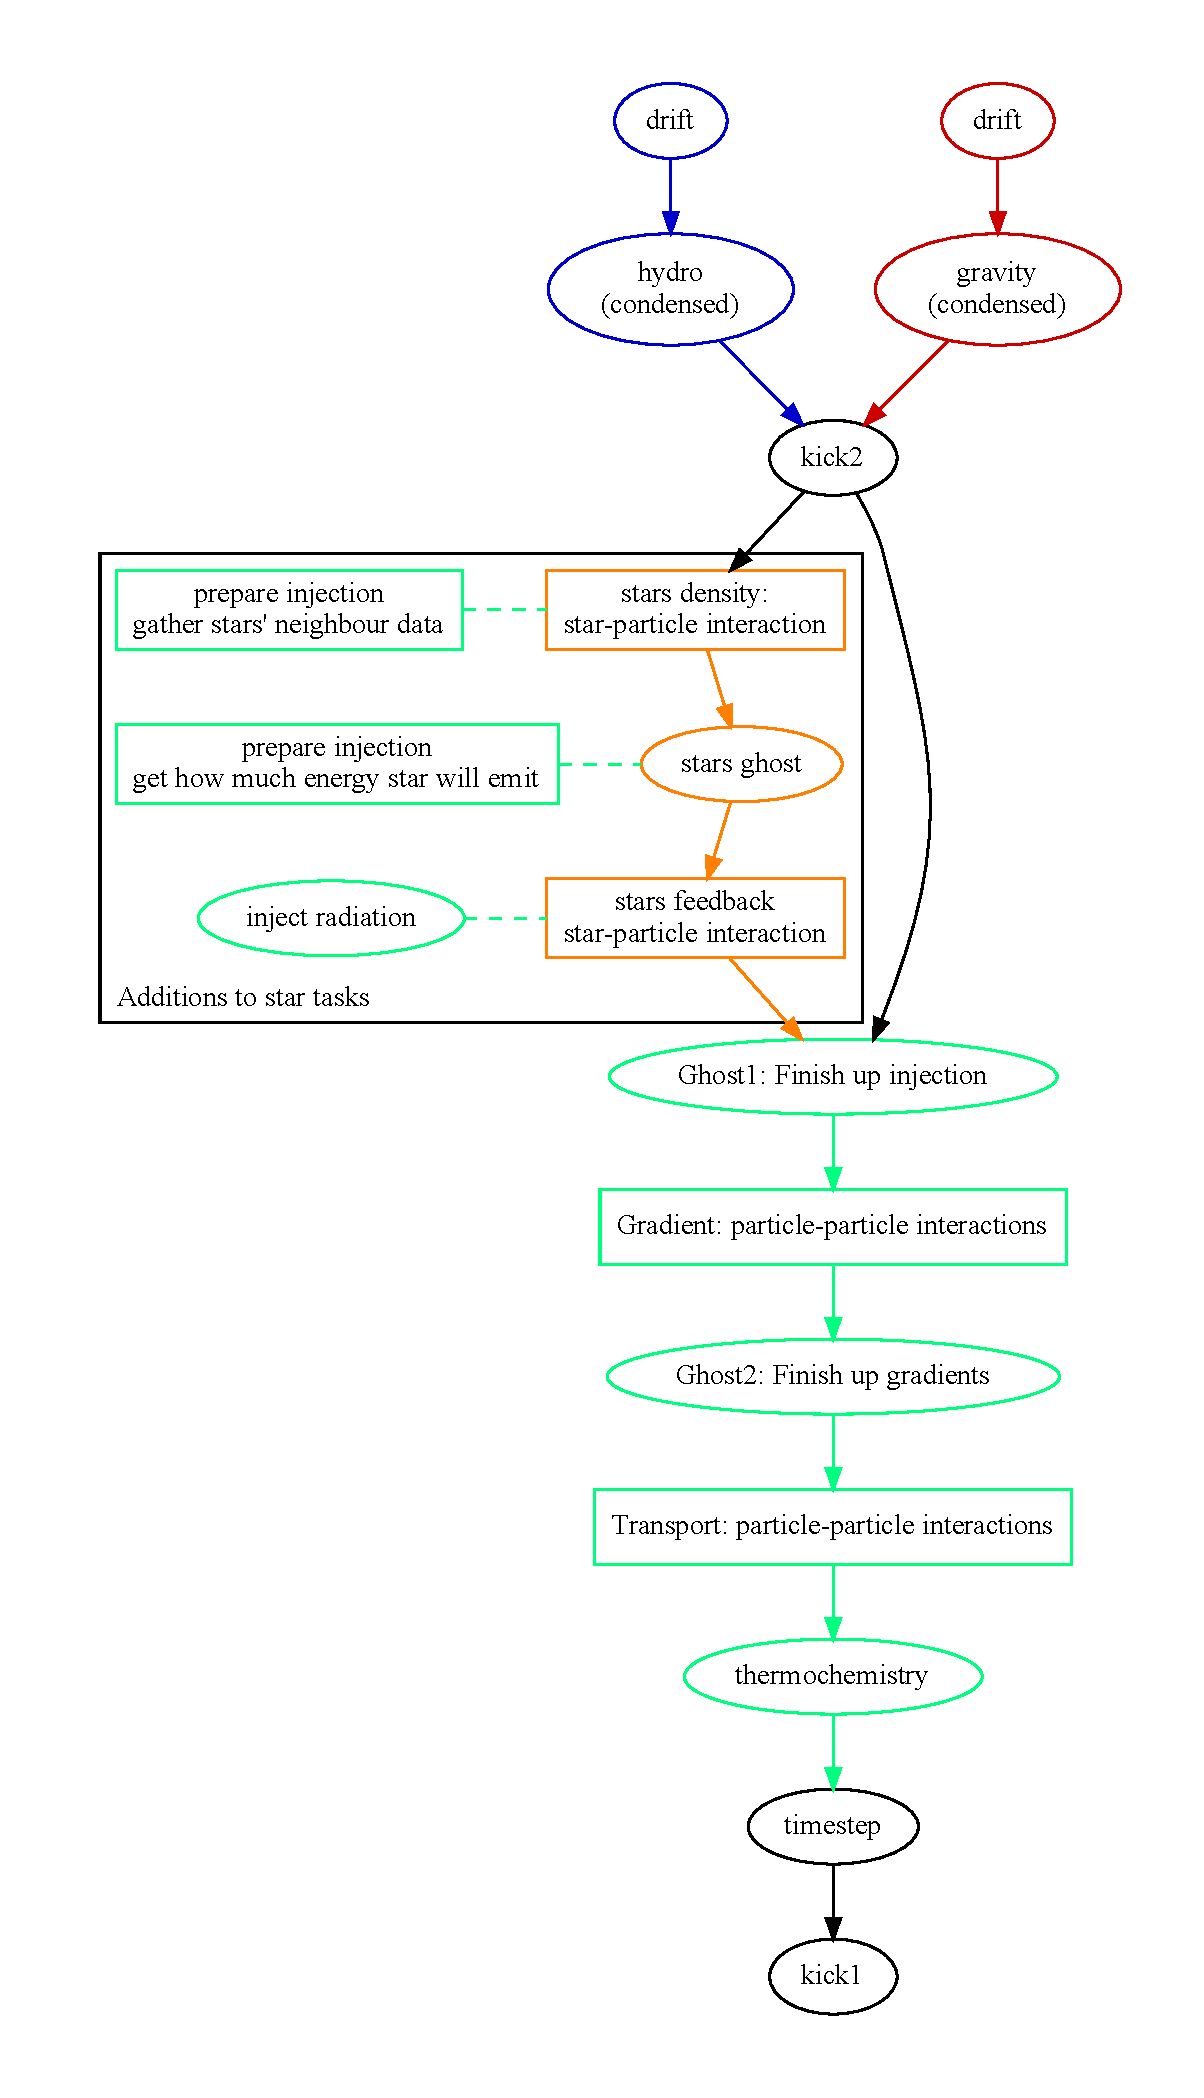
\includegraphics[width=.8\textwidth]{figures/RHD/RTTaskDependencies-simplified.pdf}%
 \caption{
A simplified task dependency graph of the tasks required for RT in \swift. For the sake of clarity,
the tasks required for the hydrodynamics and gravity have been condensed into a single node each.
Nodes with round boundaries represent \lingo{plain} type tasks, while nodes with rectangular
edges represent \lingo{interaction} type tasks.
 }
 \label{fig:RTtaskplot-simplified}
\end{figure}



\begin{figure}
 \centering
 \includegraphics[angle=90,height=.9\textheight]{figures/RHD/dependency_graph_nosubcycling.pdf}%
 \caption{
The full task dependency graph required for radiative hydrodynamics with \swift. Gravity has been
condensed into a single task.
 }
 \label{fig:RTtaskplot-nosubcycling}
\end{figure}






%------------------------------------------------------------
\subsection{Sub-Cycling}\label{chap:subcycling}
%------------------------------------------------------------



\begin{figure}
 \centering
 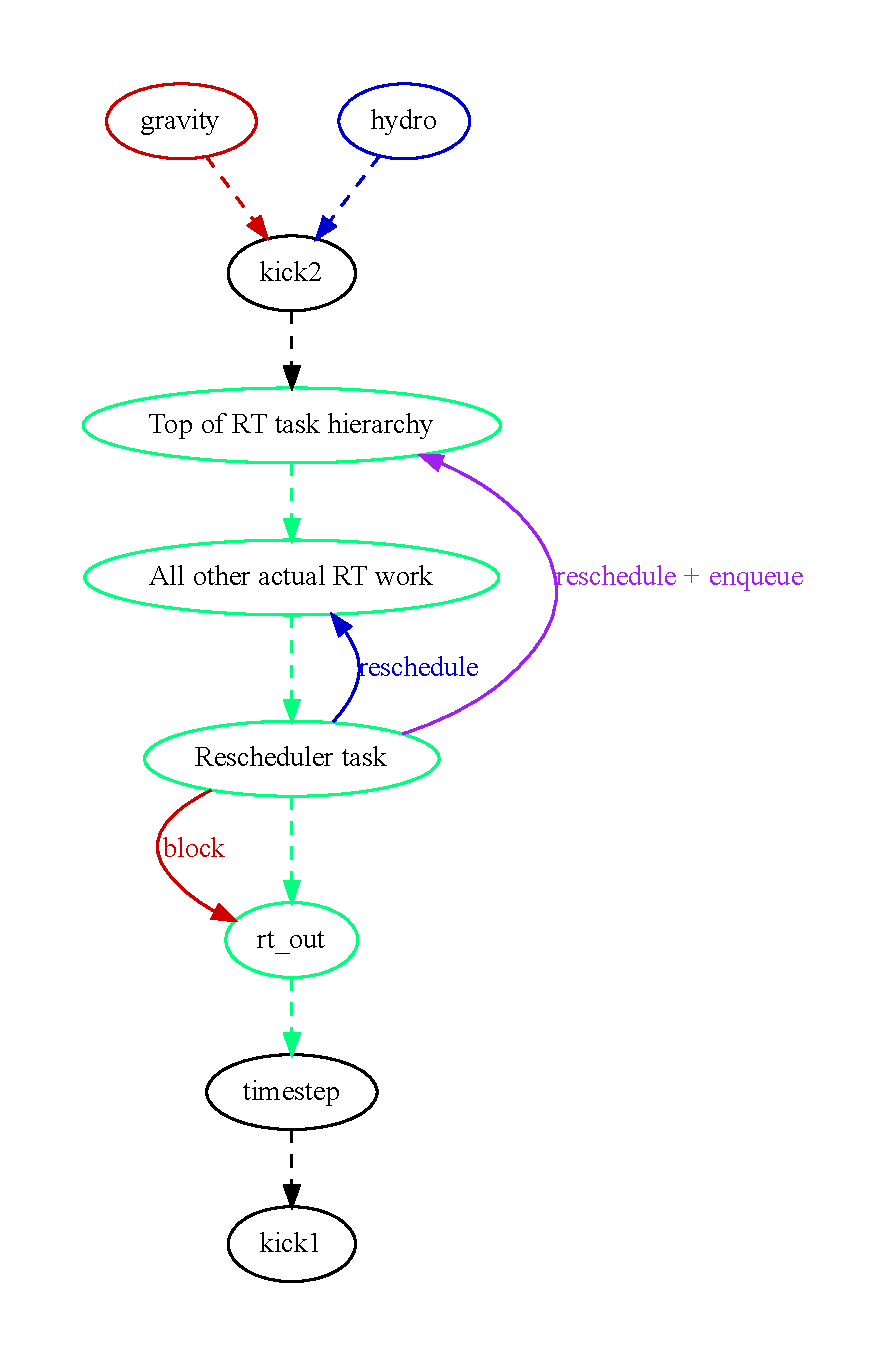
\includegraphics[width=.6\textwidth]{figures/RHD/RTRescheduling.pdf}%
 \caption{
 Illustration of the rescheduling approach for sub-cycling.  A new ``\lingo{rescheduler}'' task is
added, which blocks tasks beyond the scope of the RT block to proceed until the correct number of
sub-cycles has been completed. Instead, it sets the entire RT block of tasks to the correct state
to be executed again, and directly enqueues the task at the root of the RT hierarchy so the
subsequent sub-cycle can immediately start.
 }
 \label{fig:rescheduling}
\end{figure}





On the algorithmic side, sub-cycling (previously introduced in
Sections~\ref{chap:rt-numerics-outline} and \ref{chap:dynamic-sybcycling}) essentially consists of
repeating the entire RT block of tasks over and over again. This can be achieved in several ways.
The simplest solution is probably to repeatedly create the entire RT block of tasks, and concatenate
them correctly such that they are executed in sequence. By generating the entire RT block of tasks
$N$ times, up to $N$ sub-cycles can be executed. This is however not a very efficient solution. On
one hand, the scheduler would need to spend a lot of time fetching tasks that do the same thing over
and over again and adding them to the queues. Secondly, this approach can get quite expensive in
memory. A single RT block of tasks consists of two interaction loops with other cells, which
averages on 13 \lingo{pair} type tasks per loop per cell. In addition, there is a \lingo{self}-type
task per interaction loop, there are the two \lingo{ghost} tasks, the \lingo{thermochemistry} task,
and the MPI communication tasks, totaling 33 tasks per cell per RT block. If we needed several
hundred sub-cycles for thousands of cells, the memory expense and the associated overhead would rise
prohibitively high.

Since each sub-cycle requires the same tasks to be executed in the same order, an obvious
improvement would be to re-use the existing tasks of a singe RT block over and over again. This
could be done in the following manner, which is illustrated in Figure~\ref{fig:rescheduling}. A new
``\lingo{rescheduler}'' task is added, which has three functions. Firstly, it must block tasks
beyond the scope of the RT task block to be enqueued and proceed until the correct number of
sub-cycles has been completed. Secondly, it needs to set the entire RT block of tasks to the correct
state to be executed again. Finally, it must and directly enqueue the task at the root of the RT
hierarchy so the subsequent sub-cycle can start.



\begin{figure}
 \centering
 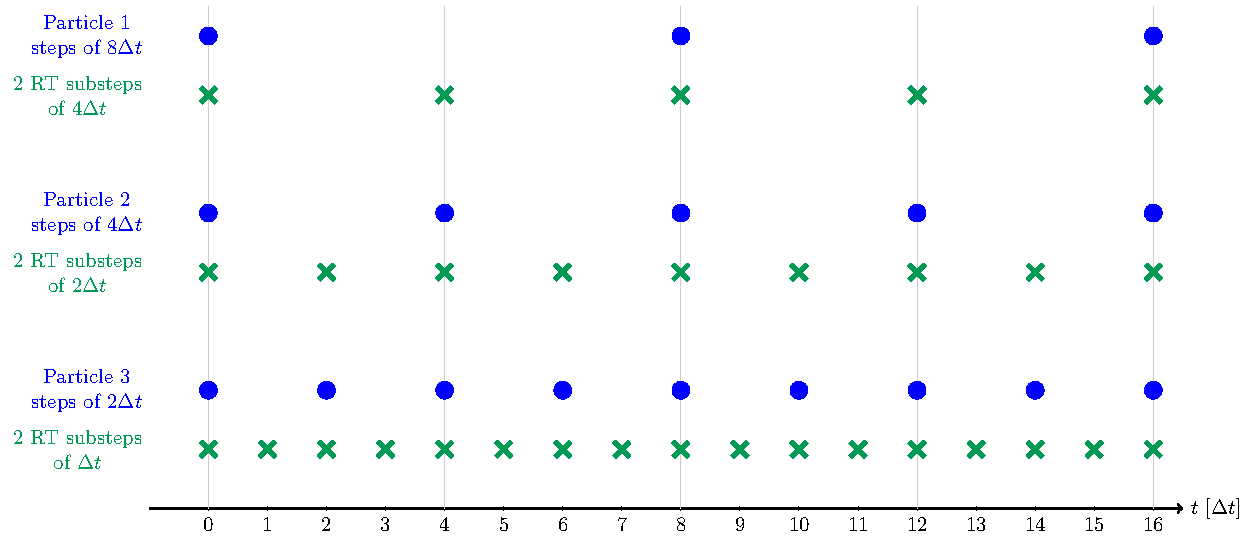
\includegraphics[width=\textwidth]{figures/RHD/two_rt_steps_per_hydro_step.pdf}%
 \caption{
The evolution of three particles with different individual time step sizes and two RT sub-cycles
each. Along the $x$-axis, the time at which the entire simulation has been advances is shown in
units of some minimal time step size $\Delta t$. Blue circles represent times at which the
particles do a hydrodynamics update. Green crosses represent the times of RT updates. Note how some
RT updates during sub-cycles overlap with global simulation times where other particles have their
regular hydrodynamics update.
 }
 \label{fig:two-subcycles-per-step}
\end{figure}




\begin{figure}
 \centering
 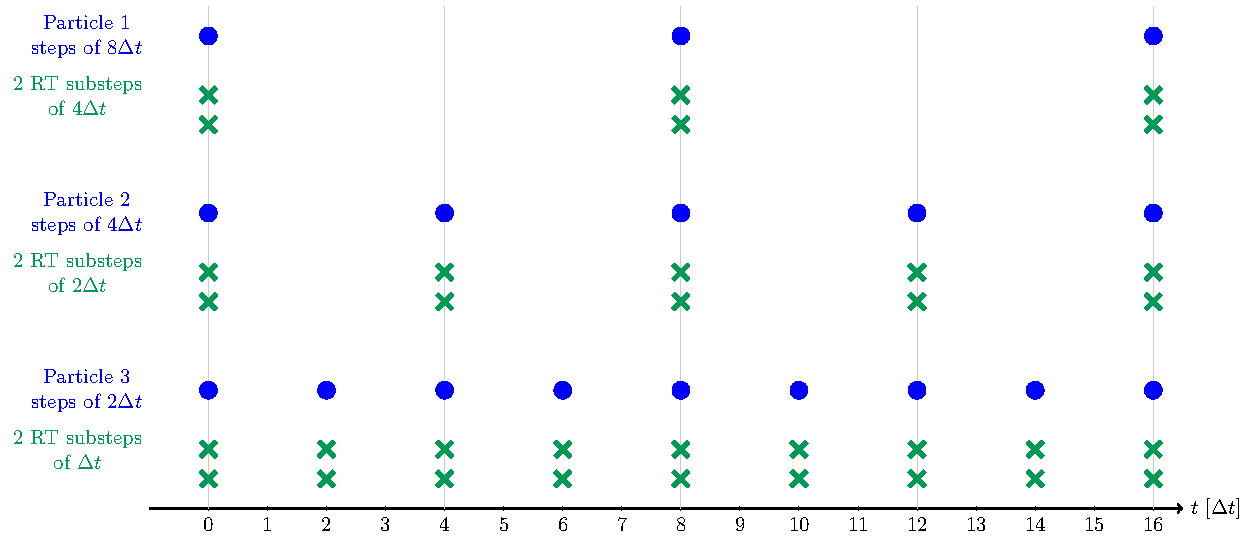
\includegraphics[width=\textwidth]{figures/RHD/rescheduler-reality.pdf}%
 \caption{
The evolution of three particles with different individual time step sizes and two RT sub-cycles
each using the rescheduling approach. Along the $x$-axis, the time at which the entire simulation
has been advances is shown in units of some minimal time step size $\Delta t$.  Blue circles
represent times at which the particles do a hydrodynamics update. Green crosses represent the times
of RT updates. Due to the nature of the re-scheduling approach, all sub-cycles of any particle must
be executed in the same global simulation step as the hydrodynamics update, even if they get
integrated in time further than the global simulation time at which they are updated. This leads to
synchronicity issues, which are shown more clearly in Figure~\ref{fig:rescheduling-problem}.
 }
 \label{fig:rescheduling-reality}
\end{figure}




A working proof of concept version of the sub-cycling through a \lingo{rescheduler} task has
successfully been developed. Unfortunately, due to the individual time step sizes of particles a
sub-cycling method using a \lingo{rescheduling} task is severely limited. To demonstrate the issues
that arise, consider the simple case where for each hydrodynamics update we do only two RT
sub-cycles. Each RT sub-cycle is then performed over exactly half the hydrodynamics time step size.
The evolution of three particles with different individual time step sizes and two RT sub-cycles
each is shown in Figure~\ref{fig:two-subcycles-per-step}. The case illustrated in
Figure~\ref{fig:two-subcycles-per-step} is actually how we want the sub-cycling to proceed: The RT
updates are performed at the appropriate global simulation times $t$. Most importantly, the RT
updates which coincide with the hydrodynamics updates of other particles with smaller hydrodynamics
time step sizes on the global simulation time axis are solved simultaneously.
%
The comparison of the time at which RT and hydrodynamics of different particles is solved is
important since the hydrodynamics for all particles needs to be solved \emph{before} the particle
can proceed with its RT updates. So the hydrodynamics update constitutes a barrier to proceed with
further RT updates. Consider for example the second RT update of Particle 2 and the second
hydrodynamics update of Particle 3 in Figure~\ref{fig:two-subcycles-per-step} should both occur on
the global simulation time $t = 2 \Delta t$. The second RT update of Particle 2 and the third RT
update of Particle 3 need to happen at the same time. For this to be possible, Particle 3 needs to
have completed its second hydrodynamics update.
%
However, this is not what a re-scheduling approach can offer. How the RT sub-cycles would be
executed with a rescheduling approach is shown in Figure~\ref{fig:rescheduling-reality}. The problem
is the fact that the rescheduling approach requires all sub-cycles to be completed in the same
global simulation step as the hydrodynamics. The rescheduling approach can only repeat all the tasks
which have been run in the current simulation step, it can not and must not advance the global
simulation time. Otherwise, it would introduce anachronisms: Some particles would be integrated
further in time than their neighbors without correctly accounting for the interactions with the
neighbor particles. This leads to very incorrect results. For example, radiation wouldn't propagate
past the particles which are \lingo{active} in that particular simulation step.

This has the consequence that data which a sub-cycling RT update requires will not be available at
the time it needs to be executed. To make use of the previous example, the second RT update of
Particle 2 in Figure~\ref{fig:two-subcycles-per-step} would need to happen at global simulation time
$t = 0$ (right after the first RT update), while the third RT update of Particle 3 is blocked by the
second hydrodynamics update, which would still occur at global simulation time $t = 2 \Delta t$.
However, these two RT updates should be happening simultaneously, as illustrated in
Figure~\ref{fig:two-subcycles-per-step}.
%
To illustrate the issue, both the case of how sub-cycling is supposed to work as well as how the
rescheduling approach would execute it are shown in Figure~\ref{fig:rescheduling-problem}. On the
top of Figure~\ref{fig:rescheduling-problem}, the intended way of sub-cycling RT updates w.r.t
hydrodynamics steps is shown. This is the same as Figure~\ref{fig:two-subcycles-per-step}, except
that three RT updates which should occur simultaneously are highlighted through arrows. At the
bottom is how the sub-cycling with a rescheduling approach would proceed. This is the same as in
Figure~\ref{fig:rescheduling-reality}, except that the same updates as in the top row are
highlighted with arrows of the same color as above. For example, the magenta arrow connects the
second RT update of Particle 1 with the third RT update of Particle 2 in both plots. The problem
with the rescheduler approach is that RT updates like the highlighted ones cannot be performed
simultaneously. On one hand, all sub-cycles must be completed before the simulation step is
finished, as in the bottom plot. But the data these highlighted RT updates require won't be
available until the simulation progresses to a further step.

The two requirements to finish all sub-cycles during a single simulation step and to have all data
available updated to the correct time unfortunately contradict each other. This can only be resolved
by abandoning individual time step sizes for particles, which is a necessity in order to be able to
run cosmological simulations to completion. As such, the rescheduling approach can't be used for
adequate sub-cycling, and we need to turn to a different solution.










\begin{figure}
 \centering
 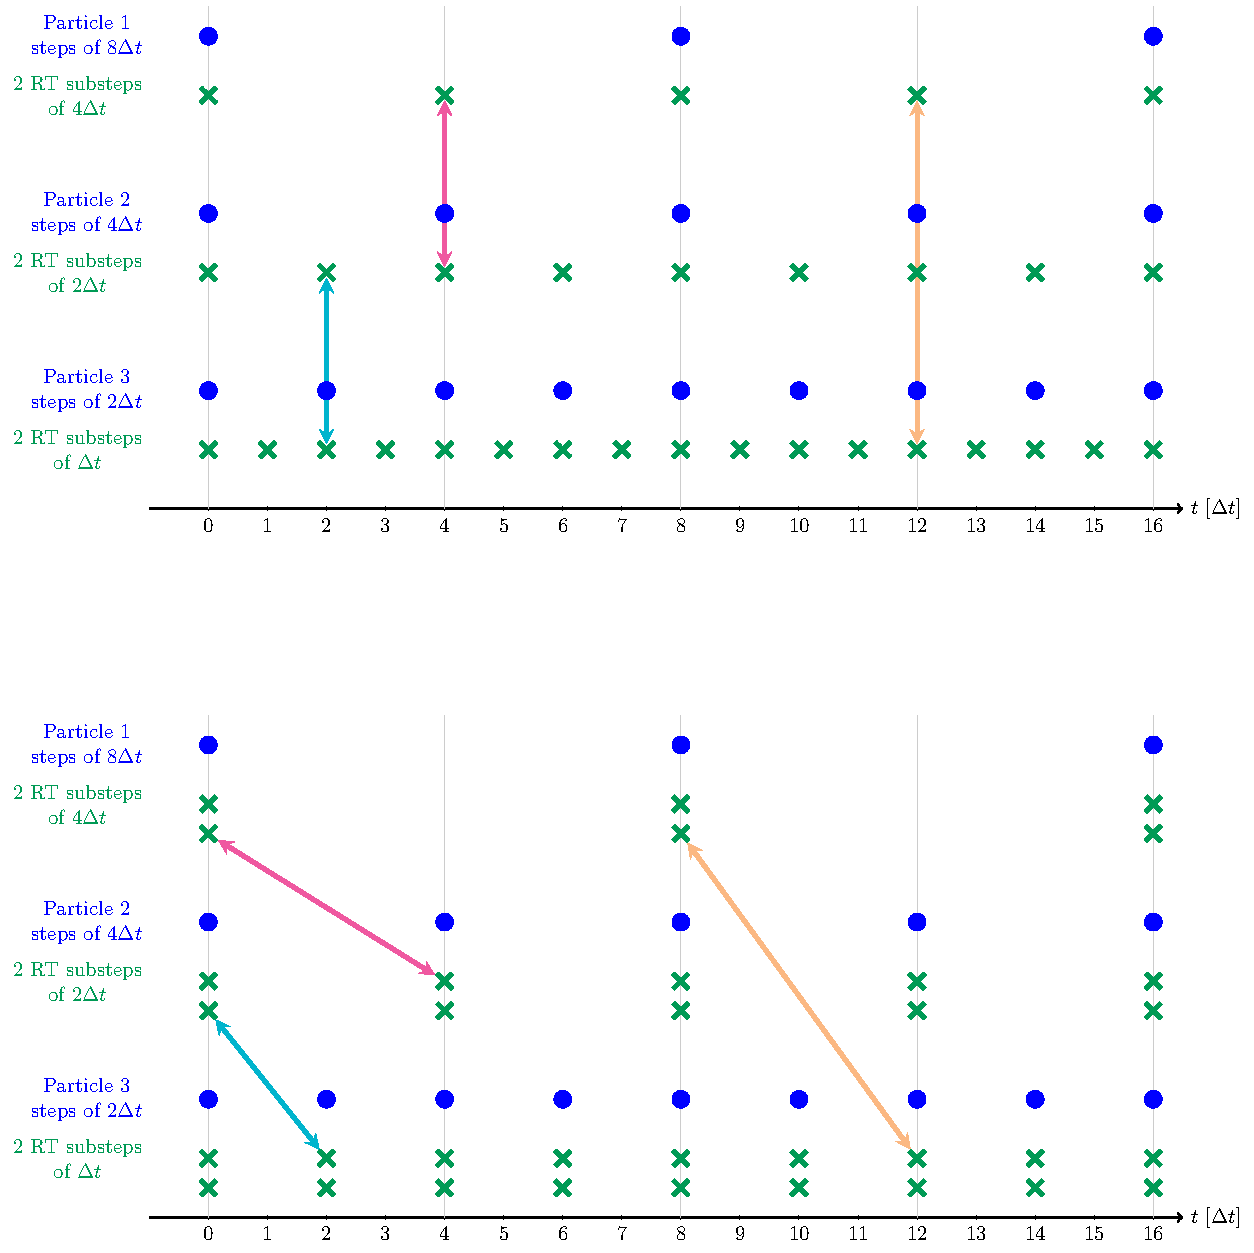
\includegraphics[width=\textwidth]{figures/RHD/rescheduler-problem.pdf}%
 \caption{
The evolution of three particles with different individual time step sizes and two RT sub-cycles
each using the rescheduling approach. Along the $x$-axis, the time at which the entire simulation
has been advances is shown in units of some minimal time step size $\Delta t$. Blue circles
represent times at which the particles do a hydrodynamics update. Green crosses represent the times
of RT updates. \\
On the top, the intended way of sub-cycling RT updates w.r.t hydrodynamics steps is shown. This is
the same as Figure~\ref{fig:two-subcycles-per-step}, except that three RT updates which should
occur simultaneously are highlighted through arrows.\\
Bottom: How the sub-cycling with a rescheduling approach would proceed. This is the same as in
Figure~\ref{fig:rescheduling-reality}, except that the same updates as in the top row are
highlighted with arrows of the same color as above. For example, the magenta arrow connects the
second RT update of Particle 1 with the third RT update of Particle 2 in both plots. The problem
with the rescheduler approach is that RT updates like the highlighted ones cannot be performed
simultaneously. On one hand, all sub-cycles must be completed before the simulation step is
finished, as in the bottom plot. But the data these highlighted RT updates require won't be
available until the simulation progresses to a further step.
 }
 \label{fig:rescheduling-problem}
\end{figure}



In order to facilitate sub-cycling alongside the use of individual time step sizes, a secondary
time marching scheme needed to be developed. To be more precise, a regular simulation step in
\swift always performs the following operations:

\begin{itemize}
 \item Activate all tasks that are attached to a cell which is active in this step
 \item Launch the scheduler and execute all tasks according to the task dependency graph
\end{itemize}

Each RT sub-cycle needs to perform these operations as well. However, during each sub-cycle, only
tasks from the RT block are \lingo{activated} and executed. In
Figure~\ref{fig:two-subcycles-per-step}, such a simulation sub-cycle step corresponds to e.g. the
update of Particle 3 at $t = \Delta t$ and $t = 3 \Delta t$, where nothing besides an RT step is
required. In addition, the sub-cycling scheme needs to be able to work concurrently alongside a
normal step. Take for example the case shown in Figure~\ref{fig:two-subcycles-per-step} at $t = 2
\Delta t$. While Particle 3 has a full hydrodynamics and RT update at that time, Particle 2 only
does an RT update. So the regular simulation step and the sub-cycling step need to be intertwined in
order to facilitate this functionality. This means that there are two classes of problems to solve:
First, sub-cycling steps between regular simulation steps need to be enabled. Second, a sub-cycling
step needs to be able to be performed during a regular simulation step.

Let's look at the sub-cycling steps between regular steps first. To facilitate this functionality,
we can exploit some peculiarities of the radiative transfer. For example, the RT doesn't drift
particles, and the signal velocity is always the (reduced) speed of light. This has the consequence
that during all sub-cycling steps, the particle's RT time step sizes always remain constant. In
other words, we know exactly how many sub-cycling steps we need to perform between two regular
steps, and can simply perform all the required sub-cycling steps in a loop. Each loop consists of
first \lingo{activating} the tasks attached to cells that contain particles which require an RT
update in that sub-cycle, and then launching the scheduler to execute all the \lingo{active} tasks
according to their respective dependencies. This launching procedure is essentially repeatedly
running regular steps for time steps determined by the sub-cycling steps, where only RT related
tasks are being \lingo{activated} and executed. One difference is a modified task dependency graph
(the modifications will be discussed further below) so the tasks related to radiative transfer can
be executed without any other tasks, in particular without hydrodynamics tasks and without the first
MPI communication in the dependency graph (\lingo{send\_xv} and \lingo{recv\_xv}). A second
difference is that cells containing particles now need to keep track of additional time and time
integration related variables for radiative transfer in order to perform the time marching and
integration correctly. This will also be discussed in more detail further below. The launching
procedure by itself however is essentially the same as for a regular step.

Before looking into the specific case where a sub-cycle's time coincides with a regular step's
time, one minor addition to the task dependency graph and to the tracking of time related variables
of cells are already necessary, as mentioned above. In order to facilitate the correct task
\lingo{activation}, cells need to store both the minimal time step size of any particle they
contain, as well as the next smallest time any particle within them will be active. Cells having
this data readily available is a general requirement for any physics, not something specific to RT
or sub-cycling. However, in order to decouple the integration times and time steps of radiative
transfer from other physics, the RT time steps and time step sizes need to be traced separately
from other now.

At the end of a step (both a regular step and a sub-cycle), i.e. after all tasks have been executed
and all active particles have been updated, the cell information needs to be updated accordingly as
well to store the up-to-date minimal time step size within them and the next smallest time any
particle within them will be \lingo{active}. In regular simulation steps, this is done in
\lingo{timestep} tasks, where the new particle time step sizes are also being computed according to
the CFL condition (eq.~\ref{eq:meshless-cfl} for hydrodynamics, and eq.~\ref{eq:rt-cfl} for RT).
Since the \lingo{timestep} tasks aren't executed during sub-cycles, a replacement task named
``\lingo{rt\_advance\_cell\_time}'' needs to be added. Note that \lingo{rt\_advance\_cell\_time}
tasks only update the cell metadata on the time step sizes they contain, not the particles within
the cells, as the time step sizes of particles don't change during sub-cycles. Similarly, a
replacement for \lingo{collect} tasks, which propagate the same time step metadata of a cell from
the \lingo{super level} to the \lingo{top level} in the cell tree hierarchy, is necessary, and has
been added as ``\lingo{rt\_collect}'' tasks. The  \lingo{rt\_advance\_cell\_time} and
\lingo{rt\_collect} tasks are shown in the final task dependency plot in
Figure~\ref{fig:RTtaskplot}.


Now let's turn to the case where a sub-cycling step overlaps with a regular simulation step.
Specifically, this means that during a regular simulation step some cells only execute the RT block
of tasks, while others do other physics as well. Complications arise here because some key
assumptions in \swift's task dependency scheme are violated. In particular, it is assumed that a
regular step in the context of hydrodynamics always starts with particle drifts, after which
particles are being sorted along the axes of active neighbor cells. If a cell is foreign, its root
of the task dependency graph starts with a \lingo{recv\_xv} task, where the (drifted) particle
positions are being received from the ``\lingo{real}'' cell. After the particle data is received,
the cell is sorted along the axes of active neighbor cells. All this doesn't take place if the cell
in question is currently doing a sub-cycle, not a regular simulation step. As particles are not
drifted in RT sub-cycles, there is no need to sort them. In the case of a sub-cycle being executed
during a regular step, the root of the task dependency graph for a cell starts with either RT tasks,
or star tasks, provided there are neighboring cells which contain star particles. In other words,
the crucial \lingo{recv\_xv} and \lingo{sort} tasks are skipped for \lingo{foreign} cells.

The missing \lingo{recv\_xv} tasks are actually not a very big problem. Since communications in
\swift always send all particle data, the first communication in the RT block, the
\lingo{recv\_rt\_gradient} tasks, will ensure that up-to-date data is available. However, the
missing \lingo{sort} task needs to be compensated with a new \lingo{rt\_sort} task which runs
after the \lingo{recv\_rt\_gradient} task is completed. Furthermore, the \lingo{rt\_sort} task  is
only \lingo{activated} if the regular \lingo{sort} task isn't. Note that since particles aren't
drifted outside of regular simulation steps, there is no need for sorts outside of sub-cycles which
coincide with regular simulation steps. The full task dependency graph required for \GEARRT which
includes sub-cycling is shown in Figure~\ref{fig:RTtaskplot}.


A final constraint that should be noted is that since the sub-cycling effectively works like a
secondary time stepping machinery, the same restriction for individual time step sizes apply. In
particular, the radiation time step sizes must be a power-of-two fraction of the maximally
permitted time step size. This requirement can be translated to demanding that the number of
RT sub-cycles a particle performs must be a power-of-two fraction of its hydrodynamics time step
size.








\begin{figure}
 \centering
 \includegraphics[angle=90,height=.9\textheight]{figures/RHD/dependency_graph_full.pdf}%
 \caption{
The full task dependency graph required for radiative hydrodynamics and sub-cycling with \swift.
Gravity has been condensed into a single task. To update cell times correctly, the
\lingo{rt\_advance\_cell\_time} and \lingo{rt\_collect} tasks needed to be added. Since with the
sub-cycling a cell may be drifted during a main step for a variety of reasons, the particles may not
have been sorted due to no particle being active in that cell in the current step. For this reason,
an additional \lingo{rt\_sorts} task has been added, which is only activated if no regular
\lingo{sort} task has been run in the current regular step.
 }
 \label{fig:RTtaskplot}
\end{figure}






